\documentclass[runningheads]{llncs}
% \IEEEoverridecommandlockouts

%\usepackage{geometry}
%\geometry{
%  a4paper,         % or letterpaper
%  textwidth=15cm,  % llncs has 12.2cm
%  textheight=24cm, % llncs has 19.3cm
%  heightrounded,   % integer number of lines
%  hratio=1:1,      % horizontally centered
%  vratio=2:3,      % not vertically centered
%}

\def\BibTeX{{\rm B\kern-.05em{\sc i\kern-.025em b}\kern-.08em
    T\kern-.1667em\lower.7ex\hbox{E}\kern-.125emX}}

%%%%%%%%%%%%%%%%%%%%%%%%%%%%%%%%%%%%%%%%%%%%%%%%%%%%%%%%%%%%%%%%%%%%%%%%%%%%%%%%
%               PACKAGES AND OPTIONS
%%%%%%%%%%%%%%%%%%%%%%%%%%%%%%%%%%%%%%%%%%%%%%%%%%%%%%%%%%%%%%%%%%%%%%%%%%%%%%%%

% Use \PassOptionsToPackage here to pass options to packages already included in 
% acmart.cls.

% Avoiding imports of commonly used packages
% ------------------------------------------------------------------------------

\usepackage{amsmath,amsfonts,mathrsfs}% for math
\usepackage{stmaryrd}                 % for special math fonts
\usepackage{float,subcaption} % for figures
\usepackage[hyphens]{url}
\usepackage[
    colorlinks,
    urlcolor=blue,
    citecolor=teal,
    linkcolor=magenta,
    ]{hyperref}                 % for hyperlinks
\usepackage{booktabs,makecell}        % for tables
\usepackage[labelfont=bf]{caption} % vil hack parce qu'on ne trouve pas pourquoi Fig est pas bold
 
% Packages for specific use
% ------------------------------------------------------------------------------

% lists and enumerations
\usepackage[inline,shortlabels]{enumitem}
% theorems definitions
%\usepackage{amsthm}
% cross-references
\usepackage{cleveref}
\usepackage{suffix}
% abbreviations
\usepackage{xspace}
% balancing columns
\usepackage{balance}
% better typsetting
\usepackage{microtype}
% other symbols
\usepackage{textcomp}

% Other packages and options
% ------------------------------------------------------------------------------

%% Glossary
\usepackage[acronym]{glossaries}
\glsdisablehyper % disable the hyperlinks
\makenoidxglossaries

%% Bibliography
\RequirePackage[
    %datamodel=acmdatamodel,
    backend=biber,
    style=lncs,
    natbib,
    mincitenames=1,
    maxcitenames=1,
    uniquelist,
    doi=false,
    url=false,
    sorting=none,
    maxbibnames=10,
]{biblatex}

%\addbibresource{bibliography.bib}
%\addbibresource{trust-fids.bib}
%\addbibresource{bib-pm.bib}
%\addbibresource{bib-leo.bib}

%https://tex.stackexchange.com/questions/41821/creating-bib-file-containing-only-the-cited-references-of-a-bigger-bib-file
\addbibresource{main-lncs_biber.bib}

% link DOI or URL if available
\newbibmacro{string+doi}[1]{%
  \iffieldundef{doi}{%
  	\iffieldundef{url}{
  		#1
	}{
		\href{\thefield{url}}{#1}
	}
  }{
  	\href{http://dx.doi.org/\thefield{doi}}{#1}
   }
  }

% on the title, in color
\DeclareFieldFormat
[article,inproceedings,inbook,incollection,patent,thesis,unpublished,misc,techreport]
  {title}{\usebibmacro{string+doi}{#1\addperiod}}

% Algorithms
\usepackage{algorithm}
\usepackage{algpseudocodex}

% Tables
\usepackage{tabularx}
\usepackage{multirow}

%Images / svg
\usepackage{svg}

% plot 
\usepackage{pgfplots}
\pgfplotsset{compat=1.18}

%tikz
\usepackage{tikz}
\usetikzlibrary{calc}

% Graphs and subgraphs
\usepackage{subcaption,graphicx}

% Properly spaced abbreviations, taken from the CVPR's style
% package (https://stackoverflow.com/a/39363004).
% Adds a period to the end of an abbreviation unless there's one
% already, then \xspace.
\makeatletter
\DeclareRobustCommand\onedot{\futurelet\@let@token\@onedot}
\def\@onedot{\ifx\@let@token.\else.\null\fi\xspace}
\def\eg{\emph{e.g}\onedot} \def\Eg{\emph{E.g}\onedot}
\def\ie{\emph{i.e}\onedot} \def\Ie{\emph{I.e}\onedot}
\def\cf{\emph{c.f}\onedot} \def\Cf{\emph{C.f}\onedot}
\def\etc{\emph{etc}\onedot} \def\vs{\emph{vs}\onedot}
\def\wrt{w.r.t\onedot} \def\dof{d.o.f\onedot}
\def\etal{\emph{et al}\onedot}
\makeatother

% \needref command
\newcommand{\needref}{\textbf{[?]}\xspace}

% Special block definition
% ------------------------------------------------------------------------------
% aglorithmic block definitions (https://github.com/chrmatt/algpseudocodex/issues/3)
\algnewcommand\algorithmicwith{\textbf{with}}%

\makeatletter
\algdef{SE}[WITH]{With}{EndWith}[1]{\algpx@startCodeCommand\algpx@startIndent\algorithmicwith\ #1\ \algorithmicdo}{\algorithmicend\ \algorithmicwith}%
\ifbool{algpx@noEnd}{%
  \algtext*{EndWith}%
  %
  % end indent line after (not before), to get correct y position for multiline text in last command
  \apptocmd{\EndWith}{\algpx@endIndent}{}{}%
}{}%

\pretocmd{\With}{\algpx@endCodeCommand}{}{}

% for end commands that may not be printed, tell endCodeCommand whether we are using noEnd
\ifbool{algpx@noEnd}{%
  \pretocmd{\EndWith}{\algpx@endCodeCommand[1]}{}{}%
}{%
  \pretocmd{\EndWith}{\algpx@endCodeCommand[0]}{}{}%
}%
\makeatother

% Tables
% ------------------------------------------------------------------------------

\newcommand{\ccell}[1]{\multicolumn{1}{c}{#1}}

% File inputs
% ------------------------------------------------------------------------------

% Notation macros
%%%%%%%%%%%%%%%%%%%%%%%%%%%%%%%%%%%%%%%%%%%%%%%%%
%% Text macros                                 %%
%%%%%%%%%%%%%%%%%%%%%%%%%%%%%%%%%%%%%%%%%%%%%%%%%

% Name of the contribution. Replace here to make 
% it effective all over the document.
\newcommand{\thecontrib}{\texttt{Trust-FIDS}\xspace}
\newcommand{\codeurl}{\url{https://github.com/<REDACTED>}}

%%%%%%%%%%%%%%%%%%%%%%%%%%%%%%%%%%%%%%%%%%%%%%%%%
%% Math macros                                 %%
%%%%%%%%%%%%%%%%%%%%%%%%%%%%%%%%%%%%%%%%%%%%%%%%%

% Notes about xparse
% Syntax: \NewDocumentCommand {name} {arguments} {body}
%   name: the name of the command
%   arguments: the arguments of the command, separated by spaces, eg. { o o m }.
%     In the argument list, o means optional, m means mandatory. Arguments can 
%     be accesesd with #1, #2, etc. Optional arguments can be provided with a
%     default value, eg. { O{default} }.
%       
\usepackage{xparse}

% \mathdef is a macro that will be used to define new macros that will be used in
%   math mode, without impacting the default behavior of the macro in text mode.
%   The macro is defined as a command that takes 3 arguments:
%     1. The name of the macro to be defined
%     2. The arguments of the macro to be defined, following the same syntax as
%        defined in xparse
%     3. The body of the macro to be defined

\DeclareDocumentCommand{\mathdef}{ m O{ } m }{%
  \expandafter\let \csname old\string#1\endcsname=#1
  \expandafter\NewDocumentCommand \csname new\string#1\endcsname { #2 }{#3}
  \DeclareRobustCommand #1 {%
    \ifmmode
      \expandafter\let\expandafter\next\csname new\string#1\endcsname
    \else
      \expandafter\let\expandafter\next\csname old\string#1\endcsname
    \fi
    \next
  }%
}

% ----------------------------
% Fedeted Learning
% ----------------------------

% Participant #1, defaults to i
\mathdef{\p}[ O{i} ]{p_{#1}}
% Number of participants, probably useless.
\mathdef{\n}{n}
% Set of all participants, same
\mathdef{\P}{P}
% Local dataset of participant $p_#1$, defaults to i
\mathdef{\d}[ O{i} ]{d_{#1}}
% Union of all local datasets
\mathdef{\D}{D}

% ----------------------------
% Clustering
% ----------------------------

% Cluster $k$ at round $r$
\mathdef{\c}[ O{k} O{r} ]{C_{#1}^{#2}}
% Number of clusters at round $r$
\mathdef{\m}[ O{r} ]{m^{#1}}
% Center of cluster k at round $r$
\mathdef{\center}[ O{k} O{r} ]{\mu_{#1}^{#2}}
% Set of clusters at round $r$
\mathdef{\C}[ O{r} ]{\mathscr{C}^{#1}}
% Distance between $p_i$ and $p_j$
\mathdef{\pdist}[ O{i} O{j} O{r} ]{\delta_{{#1},{#2}}^{#3}}
% Distance from cluster $k$ and $\ell$ centers at round $r$
\mathdef{\kdist}[ O{k} O{\ell} O{r} ]{\Delta_{{#1},{#2}}^{#3}}
\mathdef{\mdist}[ O{r} ]{\overline{\Delta^{#1}}}

\renewcommand{\Pr}{\mathbb{P}}

% ----------------------------
% Models
% ----------------------------

% Local model of participant $i$ at round $r$
\mathdef{\w}[ O{i} O{r} ]{w_{#1}^{#2}}
% Local model of participant $i$ weight in aggregation at round $r$
\mathdef{\weight}[ O{i} O{r} ]{\rho_{#1}^{#2}}
% All local models from participants at round $r$
\mathdef{\W}[ O{r} ]{W^{#1}}
% Global model for cluster $c_k^r$ at round $r$
\mathdef{\wbar}[ O{k} O{r} ]{\overline{w}_{#1}^{#2}}
% All cluster models at round $r$
\mathdef{\Wbar}[ O{r} ]{\overline{W}^r}

% ----------------------------
% Evaluations
% ----------------------------

% Evaluation of $w_j^r$ using $p_i$ local dataset $d_i$
\mathdef{\e}[ O{i} O{j} O{r} ]{e_{{#1},{#2}}^{{#3}}}
% Matrix of all evaluations at round $r$; of size $n \times n$
\mathdef{\E}[ O{r} ]{E^{#1}}
% $p_i$ evaluation on every participant at round $r$
\mathdef{\issue}[ O{i} O{r} ]{E^{#2}_{[{#1},*]}}
% Participants evaluations on $p_j$ at round $r$
\mathdef{\rece}[ O{j} O{r} ]{E^{#2}_{[*,{#1}]}}
% $p_i$ evaluation on every participant at round $r$
\mathdef{\evals}[ O{i} O{j} O{r} ]{E_{{#1},{#2}}^{{#3}}}

% ----------------------------
% Repuation
% ----------------------------
\mathdef{\Prob}[]{\vec{\mathbb{P}}}
\mathdef{\prob}[ O{q} ]{\mathbb{P}\{{#1}\}}
\mathdef{\cond}[ O{s} ]{\mathbb{P}\{\varepsilon_s|\vec{\gamma^r}\}}

\mathdef{\rep}[ O{i} O{r}]{\psi_{#1}^{#2}}


% TODO retester mathbb avec ACM. 
% Glossary content
% ---------------------------------------------------------------------------- %
% -  Thesis Glossary                                                         - %
% ---------------------------------------------------------------------------- %

%
% Acronyms
% 
% -- Examples:
% \newacronym{rssi}{RSSI}{Received Signal Strength Indication}
% \newacronym[plural=AP, longplural=Access Points]{ap}{AP}{Access Point}
% \newacronym[longplural=besoins non-exprimés]{bne}{BNE}{besoin non-exprimé}
\newignoredglossary{hidden}


% General
\newacronym[longplural={information technologies}]{it}{IT}{information technology}
\newacronym[longplural={operational Technologies}]{ot}{OT}{operational technology}
\newacronym{sdn}{SDN}{software-defined networking}
\newacronym{hr}{HR}{human resources}

% Domains
\newacronym{av}{AV}{autonomous vehicles}
\newacronym{gnb}{gNB}{next generation node base station}


% Mobile networls

% Security
\newacronym{ids}{IDS}{intrusion detection system}
\newacronym{nids}{NIDS}{network-based intrusion detection system}
\newacronym{hids}{HIDS}{host-based intrusion detection system}
\newacronym{ddos}{DDoS}{distributed denial of service}
\newacronym{dos}{DoS}{denial of service}
\newacronym{cia}{CIA}{confidenciality, integrity, availability}
\newacronym{waf}{WAF}{web application firewall}
\newacronym{ips}{IPS}{intrusion prevention system}
\newacronym{aaa}{AAA}{authentication, authorization, and accounting}
\newacronym{siem}{SIEM}{security information management system}
\newacronym{tee}{TEE}{trusted execution environment}
\newacronym{mtd}{MTD}{moving-target defense}
\newacronym{cids}{CIDS}{collaborative intrusion detection system}
\newacronym{mpc}{MPC}{multi-party computation}
\newacronym{soc}{SOC}{security operation center}
\newacronym{ad}{AD}{anomaly detection}
\newacronym{md}{MD}{misuse detection}
\newacronym{xss}{XSS}{cross-site scripting}
\newacronym{mitm}{MitM}{man-in-the-middle}

% Architectures
\newacronym{mape-k}{MAPE-K}{monitor-Analyze-plan-execute plus knowledge}
\newacronym{spof}{SPoF}{single point-of-failure}
\newacronym{smgw}{SMGW}{secure mediation gateway}
\newacronym{p2p}{P2P}{peer-to-peer}
\newacronym{mec}{MEC}{mobile edge-computing}
\newacronym{stin}{STIN}{satellite-terrestrial integrated network}
\newacronym{vm}{VM}{virtual machine}

% Networking
\newacronym{vpn}{VPN}{virtual private network}
\newacronym{mud}{MUD}{manufacturer usage description}
\newacronym{iat}{IAT}{inter-arrival time}

% I/IoT
\newacronym{ics}{ICS}{industrial control system}
\newacronym[plural=IoTs]{iot}{IoT}{Internet of Things}
\newacronym{iiot}{IIoT}{industrial Internet of Things}
\newacronym{cps}{CPS}{cyber-physical system}
\newacronym{mas}{MAS}{multi-agent systems}
\newacronym{momas}{MOMAS}{multi-objective multi-agent system}
\newacronym{bms}{BMS}{building management system}
\newacronym{plc}{PLC}{programmable logic controller}
\newacronym{siot}{SIoT}{social IoT}
\newacronym{ms}{\(\mu\)S}{microservice}
\newacronym{manet}{MANET}{mobile ad-hoc network}

% CTI
\newacronym[longplural={techniques, tactics, and procedures}]{ttp}{TTP}{techique, tactic, and procedure}
\newacronym{tti}{TTI}{technical threat intelligence}
\newacronym{cti}{CTI}{cyber threat intelligence}
\newacronym{ti}{TI}{threat intelligence}
\newacronym{apt}{APT}{advanced persistent threat}
\newacronym[plural=IoCs, longplural=Indicators of Compromise]{ioc}{IoC}{indicator of compromise}
\newacronym{stix}{STIX}{Structured Threat Information Expression}
\newacronym{taxii}{TAXII}{Trusted Automated eXchange of Indicator Information}


% Math and stats
\newacronym{iid}{IID}{independent and identically distributed}
\newacronym{niid}{non-IID}{non-independent and identically distributed}
\newacronym{pca}{PCA}{Principal Component Analysis}

% ML
\newacronym{ml}{ML}{machine learning}
\newacronym{ai}{AI}{artificial intelligence}
\newacronym{dm}{DM}{Decision-Making}
\newacronym{ddm}{DDM}{distributed decision-making}
\newacronym{svm}{SVM}{Support Vector Machine}
\newacronym{lsvm}{LSVM}{Linear Support Vector Machine}
\newacronym{cdw}{CDW}{centroid distance weighted}
\newacronym{rf}{RF}{random forest}
\newacronym{gmm}{GMM}{Gaussian mixture model}
\newacronym{sgd}{SGD}{stochastic gradient descent}
\newacronym{gd}{GD}{gradient descent}
\newacronym{lr}{LR}{logistic regression}
\newacronym{birch}{BIRCH}{balanced iterative reducing and clustering using hierarchies}
\newacronym{tl}{TL}{transfer learning}
\newacronym{mtl}{MTL}{multi-task learning}
\newacronym{elm}{ELM}{Extreme Learning Machine}
\newacronym{rl}{RL}{reinforcement learning}
\newacronym{dt}{DT}{decision tree}
\newacronym{knn}{KNN}{K-nearest neighbors}



% DL
\newacronym{dl}{DL}{deep learning}
\newacronym{drl}{deep RL}{deep reinforcement learning}
\newacronym{sda}{SDA}{stacked denoising autoencoders}
\newacronym{nn}{NN}{neural network}
\newacronym{dnn}{DNN}{deep neural network}
\newacronym{cnn}{CNN}{convolutional neural network}
\newacronym{rnn}{RNN}{recurrent neural network}
\newacronym{mlp}{MLP}{multilayer perceptron}
\newacronym{gru}{GRU}{gated recurrent unit}
\newacronym{gan}{GAN}{generative adversarial networks}
\newacronym{sfl}{SFL}{segmented federated learning}
\newacronym{dqn}{DQN}{deep Q-network}
\newacronym{bnn}{BNN}{Binarized Neural Network}


% FL
\newacronym{fl}{FL}{federated learning}
\newacronym{cdfl}{CD-FL}{cross-device federated learning}
\newacronym{csfl}{CS-FL}{cross-silo federated learning}
\newacronym{fml}{FML}{federated mimic learning}
\newacronym{hfl}{HFL}{horizontal federated learning}
\newacronym{vfl}{VFL}{vertical federated learning}
\newacronym{ftl}{FTL}{federated transfer learning}

% Evaluation
\newacronym{tpr}{TPR}{true positives rate}
\newacronym{fpr}{FPR}{false positives rate}
\newacronym{tnr}{TNR}{true negative rate}
\newacronym{fnr}{FNR}{false negative rate}
\newacronym{ppv}{PPV}{positive predictive value}
\newacronym{roc}{ROC}{receiver operating characteristic}
\newacronym{mcc}{MCC}{Matthews correlation coefficient}
\newacronym{mse}{MSE}{mean squared error}

% Distributed Leadgers
\newacronym{auc}{AUC}{area under the curve}
\newacronym[longplural=distributed ledger technologies]{dlt}{DLT}{distributed ledger technology}
\newacronym{dag}{DAG}{directed acyclic graph}

% Technical solutions
\newacronym{swat}{SWaT}{Secure Water Treatment}
\newacronym{iads}{IADS}{Intrusion and Anomaly Detection System}
\newacronym{vsl}{VSL}{Virtual State Layer}
\newacronym{rsu}{RSU}{roadside unit}
\newacronym{v2x}{V2X}{vehicle-to-everything}

% Conferences and journals
\newacronym[type=hidden]{icccn}{ICCCN}{IEEE International Conference on Computer Communications and Networks}
\newacronym[type=hidden]{icdcs}{ICDCS}{IEEE International Conference on Distributed Computing Systems}
\newacronym[type=hidden]{cnsm}{CNSM}{International Conference on Network and Service Management}
\newacronym[type=hidden]{icecce}{ICECCE}{International Conference on Electrical, Communication, and Computer Engineering}
\newacronym[type=hidden]{bdsa}{BigDataSE}{IEEE International Conference on Big Data Science and Engineering}
\newacronym[type=hidden]{iccc}{ICCC}{IEEE/CIC International Conference on Communications in China}

% University and other research institutes
\newacronym{accs}{ACCS}{Autralian Center for Cyber Security}
\newacronym{cic}{CIC}{Canadian Institute of Cybersecurity}
\newacronym{cse}{CSE}{Communication Security Establishment}

% Research and methodology
\newacronym{slr}{SLR}{Systematic Literature Review}
\newacronym{rq}{RQ}{research question}

% Own
\newacronym{fids}{FIDS}{Federated Intrusion Detection System}


%
% Glossary
%
% -- Note: adding '%' at the end allows to break line without semantic
%
% -- Examples:
% \newglossaryentry{wifi}
% {
%     name=WI-FI,
%     plural=WI-FI,
%     description={
%         Technologie sans-fil qui permet à des appareils de communiquer entre
%         eux, notamment sur Internet%
%     }
% }




% Page numbers
% ------------------------------------------------------------------------------
%\pagestyle{plain}


% Personalized theorems
% ------------------------------------------------------------------------------

% Relax the `\proof` command used in LNCS cls causing
% "Command \proof already defined"
% Solution: https://tex.stackexchange.com/a/699868
\let\proof\relax\let\endproof\relax
\usepackage{amsthm}

%% Hypotheses
\theoremstyle{definition}
\newtheorem{hypothesis}{Hypothesis}
\crefname{hypothesis}{hypothesis}{hypotheses}
\Crefname{hypothesis}{Hypothesis}{Hypotheses}

%% Challenges
\theoremstyle{definition}
\newtheorem{challenge}{Challenge}
\crefname{challenge}{challenge}{challenges}
\Crefname{challenge}{Challenge}{Challenges}

%% Research Questions
\newtheorem{innerRQ}{RQ}
\crefname{innerRQ}{RQ}{RQs}
\Crefname{innerRQ}{RQ}{RQs}

\newenvironment{RQ}[1]
  {\renewcommand\theinnerRQ{#1}\innerRQ}
  {\endinnerRQ}

\def\changemargin#1#2{\list{}{\rightmargin#2\leftmargin#1}\item[]}
\let\endchangemargin=\endlist 

% Lorem Ipsum
\usepackage{lipsum}

% Lengths
\setlength{\intextsep}{1.5\baselineskip plus 0.2\baselineskip minus 0.2\baselineskip}
\setlength{\textfloatsep}{1.5\baselineskip plus 0.2\baselineskip minus 0.2\baselineskip}
\setlength{\floatsep}{1.5\baselineskip plus 0.2\baselineskip minus 0.2\baselineskip}

%%%%%%%%%%%%%%%%%%%%%%%%%%%%%%%%%%%%%%%%%%%%%%%%%%%%%%%%%%%%%%%%%%%%%%%%%%%%%%%%
%               DOCUMENT
%%%%%%%%%%%%%%%%%%%%%%%%%%%%%%%%%%%%%%%%%%%%%%%%%%%%%%%%%%%%%%%%%%%%%%%%%%%%%%%%

%%
%% end of the preamble, start of the body of the document source.
\begin{document}
%\title{Trust-FIDS: Distributed Cross-evaluation for Reputation-aware Model Weighting in Federated Learning
%\title{Trust-FIDS: Leveraging Cross-evaluation in Reputation Weighting in Federated Learning
%\title{Trust-FIDS: Cross-Evaluation for Collaborative Federated Learning Intrusion Detection System
%\title{Trust-FIDS: Cross-evaluation for Contribution Filtering in Federated-Learning-based Intrusion Detection
%\title{Trust-FIDS: Cross-evaluation for Contribution Filtering in Federated-Learning-based IDS
\title{Trust-FIDS: Cross-evaluation for Poisoning Mitigation in Federated-Learning-based IDS
%\thanks{%
%This research is part of the chair CyberCNI.fr with support of the FEDER development fund of the Brittany region.}
}
\titlerunning{Trust-FIDS}

\author{
     Léo Lavaur\inst{1}%\orcidID{0000-1111-2222-3333}
\and Pierre-Marie Lechevalier\inst{1}%\orcidID{1111-2222-3333-4444}
\and Fabien Autrel\inst{1}%\orcidID{2222-3333-4444-5555}
\and Yann Busnel\inst{2}%\orcidID{1111-2222-3333-4444}
\and Hélène Le~Bouder\inst{1}%\orcidID{1111-2222-3333-4444}
\and Romaric Ludinard\inst{1}%\orcidID{0000-0002-4997-4813}
\and Marc-Oliver Pahl\inst{1}%\orcidID{1111-2222-3333-4444}
\and Géraldine Texier\inst{1}%\orcidID{1111-2222-3333-4444}
}

\institute{
    IMT Atlantique / IRISA, Rennes, FRANCE\\
     \email{firstname.name@imt-atlantique.fr}\\
%\and Chair CyberCNI.fr, FRANCE\\
%     \email {\{lavaur,pahl\}@cybercni.fr}
\and 
    IMT Nord Europe / IRISA, Lille, FRANCE\\
     \email{yann.busnel@imt-nord-europe.fr}
}


\authorrunning{L. Lavaur, P-M. Lechevalier {\em et al.}}

\maketitle
%\thispagestyle{plain} % to display the page number on first page
\vspace{-1pt}
\begin{abstract}
  % (blue) Basic introduction to the field (one or two sentences): 
  %\Glspl{cids} improve resilience to distributed attack campaigns by allowing \acrshortpl{ids} to share locally acquired knowledge with peers.
  %While it consequently improves detection, data sharing is challenging, especially in \gls{ml} workflows.
  % (pink) More detailed background (Two or three s)
  %\Gls{fl} is a distributed learning paradigm that enables \glspl{cids} without the need to share local data, while still benefiting from the experience of all participants.
  The emergence of \gls{fl} has allowed \glspl{cids} to benefit from the experience of multiple actors, without disclosing local data.
  %By sharing the learning task among several actors, it allows training a global intrusion detection model that benefits from the data of all participants.
  Yet, negligent or malicious clients might negatively contribute to the global model and degrade its performance.
  % (yellow) General problem (1 s)
  %Existing mitigation strategies falter in heterogeneous settings, while \gls{cids} participants are inherently heterogeneous.
  \Glspl{cids} inherently generate and consume heterogeneous data, complicating the detection of malicious behaviors by existing mitigation strategies, which tend to falter in such settings.
  %Existing mitigation strategies tend to falter in \glspl{cids} because they generate and consume heterogeneous data, which complicates the detection of malicious behaviors.
  We present \thecontrib, a novel \gls{fl} architecture for intrusion detection able to deal with malicious contributions, even in heterogeneous settings, and without a centralized source of truth.
  %TODO personne je ne suis pas fan du we mais pluoto de la forme passive en anglais
  \thecontrib leverages client-side evaluation to cluster participants based on their similarity.
  These evaluations then feeds a reputation system that weights participants' contributions based on their perceived trustworthiness.
  We evaluate our approach on four intrusion detection datasets in various poisoning settings, and against a state-of-the-art mitigation strategy.
  Our results show that combining clustering and a reputation system succeeds in detecting both colluding and lone attackers, highlighting its versatility.
  
  % (cyan) Summarizing the main results (one s)
  %We show that our clustering successfully groups participants originating from the same dataset together, while excluding the noisiest attackers. 
  %The reputation system then strongly limits the impact of stealthier attackers, as long as they remain a minority within the cluster.
  %We show that 
  
  % (green) summarizing how the result/approach compares with past work (2 or 3 s)
  %We confront our work with a state-of-the-art poisoning mitigation approach. 
  %We show comparable performance when using a single dataset, and vastly outperform them when data originate from multiple datasets, a case we deem more realistic for \gls{cids}.  
  %The comparison of our work with a state-of-the-art mitigation strategy highlights its versatility in detecting both colluding and lone attackers. %\gls{iid}, and \acrshort{niid} data for the different attack scenarios. 
  % In particular, we outperform them on \acrshort{iid} and practical \acrshort{niid} use cases, while remaining comparable in the pathological \acrshort{niid} ones, that are less relevant for \gls{cids}. 
  
  % The comparison of our work with a state-of-the-art mitigation strategy highlights its versatility.
  % In particular, we outperform them on \acrshort{iid} and practical \acrshort{niid} use cases, while remaining comparable in the pathological \acrshort{niid} ones, that are less relevant for \gls{cids}.
  
  % (purple) Put the results in a more general context (1 or 2)
  % (red) optional perspective (2 or 3)
  %Our work is open source, and all codes will be found on a public repository in case of acceptance.%at: \codeurl. 
  %TODO LN found on on est sur du on ?

  \keywords{Federated Learning \and Intrusion Detection \and Cross-evaluation \and Similarity \and Clustering \and Reputation Systems \and Trust \and Heterogeneity}
\end{abstract}

%\begin{IEEEkeywords}
%federated learning, intrusion detection, reputation systems, trust, heterogeneity, clustering, cross-evaluation
%\end{IEEEkeywords}

%%
%% This command processes the author and affiliation and title
%% information and builds the first part of the formatted document.
%\maketitle

% Sections
% ------------------------------------------------------------------------------

%reintroduce acronyms
\glsresetall



\section{Introduction}\label{sec:intro}

%With the ever-increasing number of cyberattacks, \gls{ids} play a critical role in the protection of information systems.
%\Glspl{nids} are especially relevant for organizations, as they can detect malicious activities in large-scale information networks, such as data exfiltration or \gls{dos} attacks. 
%
%\Gls{ml} is significantly represented in the \gls{nids} literature, enabling the characterization of network traffic and detection of abnormal behaviors.
%However, these \gls{ml} algorithms require large quantities of data to be trained.
%While data-sharing between organizations could address this requirement, 
%As a result, stakeholders generally show reluctance to adopt \glspl{cids}.

For several years, the adoption of collaborative \gls{ml} has been limited by the risks induced in data-sharing.
\Glspl{nids} are especially concerned, as sharing network data can expose information about the inner workings of information systems.
The recent advances~\cite{kairouz_advances_2021} in \gls{fl} promise to solve such issues, allowing participants to collaboratively train a global model without sharing their local data~\cite{mcmahan_communication-efficient_2017}.
% - Contexte de la contribution et cas d'application du FL: conglomérat d'organisations (on cite acteurs industriels ?) ayant des exigeances de sécurité suffisament proche pour souhaiter partager des informations de détection d'intrusion.
%\Gls{fl} is a privacy-preserving distributed learning paradigm that allows 
Specifically, organizations in \glspl{cids} can leverage \gls{hfl} (\ie same features, but different samples), to share their observations with other participants while keeping their locally collected network data private~\cite{lavaur_evolution_2022}. %, thus virtually extending the size of their training set.

% - PB1: Tout systeme collaboratif s'expose à la participation d'acteurs malveillants ou simplement de bonne foi avec des données de mauvaise qualité -> créer de la confiance
Collaborative systems are especially sensitive to input quality.
For instance, malicious participants in a \gls{cids} could poison their contributions to impact the convergence of the global model, or introduce backdoors that could be exploited afterward.
Even honest participants can negatively contribute to the aggregation by training their model on data of poor quality or by being unaware of attacks present in their network.  
% - PB2: Dans un contexte fortemmet hétérogène il est difficile de distinguer une attaque d'une contribution différente du fait de ses données d'entrées.
Moreover, different organizations might exhibit substantial differences in their information systems, such as hosted services or used protocols.
This can lead to significant variations in model updates, as each organization trains its model on its local network traffic.
In this heterogeneous context, it is very difficult to distinguish a negative contribution from a legitimate one originating from a different infrastructure.

% SOA:
% -
% Approaches that aim to mitigate model poisoning typically leverage a single source of truth or model comparisons .
% They either compare  on a single source of truth \cite{blanchard_machine_2017,cao_fltrust_2022}, such as a server-maintained model or a representative training set, to compare participants' updates with.
% However, building a single source of truth is infeasible in \gls{niid} settings, due to the differences between participants.
% % - en mode "pair-wise"
% In contrast, other works compare participants' model updates with each other.
% It can be used to either remove outliers in \gls{iid} settings~\cite{yin_byzantine-robust_2018}, or detect participants that collude to poison the global model in \gls{niid} settings~\cite{fung_limitations_2020, awan_contra_2021}. 
% These \gls{niid} technics, however, fail to detect a single attacker, we also show that in case where legitimate participant look alike they can be detected as colluding participants. 

% - anti-poisoning iid
Approaches that mitigate model poisoning in homogeneous distributions typically compare or evaluate a model using a single source of truth~\cite{blanchard_machine_2017,cao_fltrust_2022}.
% KO en non-iid
Building such a single source of truth, however, is infeasible in heterogeneous contexts due to the differences between participants. 
Assuming that all contributions are different, some approaches detect colluding attackers based on their similarity~\cite{fung_limitations_2020, awan_contra_2021}. 
%By construction, 
Nevertheless, these approaches fail to detect an isolated, yet potent, attacker.
%We also show that in case where legitimate participant look alike, they can be unfairly detected as colluding participants. 


% % % - avec single source of truth
% Some rely on a single source of truth \cite{blanchard_machine_2017,cao_fltrust_2022}, such as a server-maintained model or a representative training set, to compare participants' updates with.
% However, building a single source of truth is infeasible in \gls{niid} settings, due to the differences between participants. 
% % - en mode "pair-wise"
% In contrast, other works compare participants' model updates with each other.
% It can be used to either remove outliers in \gls{iid} settings~\cite{yin_byzantine-robust_2018}, or detect participants that collude to poison the global model in \gls{niid} settings~\cite{fung_limitations_2020, awan_contra_2021}. 
% These \gls{niid} technics, however, fail to detect a single attacker, we also show that in case where legitimate participant look alike they can be detected as colluding participants. 
% However, similarity-based filtering would exclude model updates that are different, even though they are relevant to the global model.
% For instance, two models trained on different protocols can differ statistically, could maintain high accuracy on a common test set.


% % notre approache fait (présentation TRES rapide)
% % - les métriques de comparison de modèles entre eux ne sopnt pas pertyinentes (single source, model diff mais performant) -> cross-evaluation
% % - besoinde réduire l'hétérogénéité -> clustering (cite qques paiers qui en font déjà) mais en utilisant les métriques fournies par la xeval
% % - cluster ne prend pas enc compte l'historique, et risque de manquer des déviation fines -> réputation en prenant les eval comme feedback
% % - objectif: construire de la confiance par éval sucessive
% For these reasons, we present \thecontrib, a defense strategy for \gls{csfl} that relies on client-side model evaluation.
% Instead of comparing participant models on the server, we propose that participants subjectively evaluate the others' contributions. %' quality. 
% To that end, we add a new step to the typical \gls{fl} workflow, between training and aggregation, where each participant uses its local dataset to evaluate the other participants' models. 
% %Based on the result of this cross-evaluation, our approach regroups similar-looking participants together using hierarchical clustering, before weighting their model aggregation using a reputation system.
% %These evaluations are adjusted based on their historical similarity with other cluster member evaluations. 
% Our approach then leverages this \emph{cross-evaluation} to assess participants' similarity and group them using hierarchical clustering, before weighting the model aggregation using a reputation system.

In this paper, we present \thecontrib, a defense strategy for \gls{csfl} aiming at detecting attackers (colluding or not) regardless of the data homogeneity. \thecontrib relies on three main ingredients:
\begin{enumerate*}[label=\em {\roman*})]
    % \item contrarily to classical FL approaches where participants models are compared on a centralized server, we propose that participants subjectively evaluate the others' contributions. %' quality. 
% To that end, we add a new step to the typical \gls{fl} workflow, between training and aggregation, where each participant uses its local dataset to evaluate the other participants' models,
    \item a modified \gls{fl} workflow, where each participant uses its local dataset to evaluate the other participants' models, between training and aggregation steps, in contrast with classical FL approaches where participants models are compared on a centralized server,
    % \item a modified \gls{fl} workflow, where each participant evaluates the other participants' models thanks to its local dataset,
    \item participants are gathered into clusters thanks to their similarity,
    \item a reputation system is leveraged to weight participants contributions.
    %on a global model.
\end{enumerate*}

% Our evaluation shows that \thecontrib can effectively identify lone and colluding attackers in highly heterogeneous settings, while ensuring convergence of the benign participants.
We measure the performance of \thecontrib using four network flow datasets with standardized features, representing various use cases.
%We show that our clustering method can reproduce the initial distribution of participants. 
We also compare our approach to existing ones~\cite{mcmahan_communication-efficient_2017,fung_limitations_2020}, and find that \thecontrib detects attackers under most attack scenarios, including lone and colluding attackers, targeted and untargeted attacks, in different types of poisoning strategies.

% Summary
To summarize, our contributions are threefold:
%TODO LN moi je metterai des formes passives
\begin{enumerate}[label=({\arabic*})]
    \item we present \thecontrib, an architectural scheme to protect \gls{fl} strategies using clustering and reputation-aware aggregation; with an extensive evaluation under different attacks and distributions, and against relevant baselines,
    \item we show that evaluation metrics (such as accuracy, f1-score, or loss) can effectively be used to assess similarity between \gls{fl} participants, and as input to clustering algorithms,
    \item we provide a \gls{fl} reputation system, leveraging local evaluation to swiftly adapt aggregation weights and protect the system's convergence.
    %\item We compare our approach with \texttt{FoolsGold}~\cite{fung_limitations_2020}, a relevant baseline that emphasizes on detecting colluding attackers in heterogeneous contexts.
    %\item We provide extensive evaluation \thecontrib under different types of attacks and client distributions.
\end{enumerate}

%%%% §7 Leo
The rest of this paper is organized as follows.
\Cref{sec:problem} defines the addressed problem and introduces our threat model.
We detail in \Cref{sec:related} our positioning and \thecontrib's benefits over related works.
\Cref{sec:archi} presents \thecontrib's design and core components, before an extensive evaluation in \Cref{sec:eval}.
We discuss our findings in \Cref{sec:discussion} before concluding and laying out future works.




% NIDS background
%Intrusion detection refers to methods and systems that can identify potential threats in an information system.
%Sharing actionable intelligence between organizations can improve the performance of \glspl{ids}. 
%However, collaboration also brings challenges, \eg trust between parties, privacy and confidentiality and, finally, protection against poisoning~\cite{wagner_novel_2018}.
%
%Typical collaborative \gls{ml} requires all data to be centrally collected, curated, and processed.
%Sending training data to a remote server implies sending it over a network.
%Depending on the type of training data, it can represent an important bandwidth consumption, especially for \gls{nids} workflows.
% Finally, it can also mean that clients are unable to exploit their data locally, and solely rely on a remote server to provide them with t













%%%%%%%%%%%%%%%
%%%%%%%%%%%%%%%
%%%%%%%%%%%%%%%

% By only sharing the model weights instead of the underlying data or IoC federated learning limit the risk of unintentional information disclosure. 
% Traditionally, and for the sake of simplicity, the aggregation of the global model is done using the average weight from local models.
% Each local model from the participants thus have an equal impact on the global model which might not be ideal.%% TODO 2 : insérer citation, le nom de "l'algo" de base c'est FedAvg ?
% In our case, different participants might have infrastructures too diverse to make knowledge transfer between participants possible. 
% Also, compromised participants might unknowingly send inaccurate classification that end up poisoning the aggregated model.  
% Strategies that take into account the quality of the local model during the aggregation process have been shown to increase the accuracy of the global model and to converge faster.\cite{wang_reputation-enabled_2021,wang_novel_2020}

% Theses strategies usually rely on a comparison between the evaluated local model and one or multiple other models. 

%The comparison can take different forms : 
% \begin{enumerate}
%     \item It can be made against variants from the global model, e.g. the global model from the last round. Alternatively, against a temporary version of the new global model curated from the evaluated local model. \cite{wang_reputation-enabled_2021} \cite{xia_tofi_2021}
%     \item It can be a pairwise comparison with the others local models \cite{wang_flare_2022} 
%     \item Deviation from historical local models
%     \item Assessing the accuracy of the local models by testing it against a data-set located on the central actor that is in charge of the aggregation process.\cite{cao_fltrust_2022} \cite{xia_tofi_2021}. 
% \end{enumerate}
% 
% This last strategy however make the assumption that the central actor detain a part of the data set that is representative of the locals data set and are typically more aimed at IID-dataset.
% 
% In order to also address non IID-dataset, having a representative data set located on central actor is too strong of an assumption.
% 
% We try to tackle this problem by letting the participants evaluate the local models accuracy of their peer themselves. 
% 
% Based on existing work in trust and reputation we build a trust overlay to better judge the feedback that participants sent on the local models of their peers. 
% 
% The reliability of this approach is dependant on the collaboration between participants and thus on the chosen threat model that will be detailed in section TODO. 
% % TODO : lien vers la section threat model
% Aggregation strategies usually discard local models that are too different from the global model.
% Based on the hypothesis that different models might be more accurate for diverse environments we choose to cluster local models that match together instead of pruning all the deviations from the global model. 
% This effectively create several global models in which a participant local model can be aggregated. 
% 
% % Several strategies have also been suggested to measure the difference between two models : 
% % \begin{enumerate}
% %     \item cosine similarity 
% %     \item
% % \end{enumerate}
% 
% % Attention je n'ai pas mentionné l'élément différentiant qui est le fait de tester l'accuracy du modèle ches les participants plutôt que centralement ou de se baser sur un score similitude. 
% % C'est bénéfique car cela permet de ne pas avoir de données sur l'acteur centralisé et de traiter des cas non-IID. Nous sommes typiquement dans ce type de scénario car les organisations peuvent avoir des infrastructurs très différentes. 
% 
% 
% %\subsection{Use case of collaborative intrusion detection} 
% 
% The goal is to be able to detect an anomaly and an intrusion with several systems collaborating.
% We propose to use federated learning.
% 
% An entity has a global view of its network (with various devices), it has a knowledge of the traffic running on the network (pcap file for ex). 
% The goal is to learn the legacy comportment by learning it on the traffic, then it will be able to detect an anomaly (by reducing the dimension of the model). 
% It will compute the reduction of the dimension by exchanging information with other entities (organizations participating in the collaboration to detect anomalies).
% 
% The model is synchronous with rounds. 
% The system will ask the model to learn and to share its state with others involved in the collaboration.
% 
% At each round, the server shares the current model (the weight matrix). 


%%%
% Léo : détient des métriques pertinentes à observer pour savoir quelle serait l'overhead d'un tel système et les critères % de réussite.
% 
% Hypothèse :
% 	- 
% 	
% ## Evaluation système malveillant 
% - Consomation ressource 
% - Détection d'un acteur malveillant  
%  
%  Regarder plus précisement les métriques d'intérêt du point de vue du système de réputation : 
% - Acteurs malveillant. 
% - Consomation ressources.
% 
% 
% 
% Distiction de ce travail : 
% - vis à vis du feaderated learning
% - ou vis à vis de 
% 
% 
% Voir s'il y a particularité vis à vis des autres systèmes de réputation utilisés dans le federated learning ? 
% - Est-ce que l'aspect clusterisation. 
% - 
% 
% Clusterisation à partir de l'évaluation local du modèle. 
% Déviance du modèle vis à vis d'un historique. 
% Ecart du modèle : 
% 	- distance entre les deux matrices de poids. 
% 
% On peut vérifier la distance entre deux modèles parfaits. 
% 
% 
% Parcourir l'histoire du usecase : 
% 
% 
% Histoire pour le usecase :
% ### Point de vue du client
% Je (un appareil d'une organisation) reçoit des logs du traffic passant sur l'ensemble du réseau (qui peut être de taille variable) j'en apprend le comportement normal via réduction de dimmension : on trouve un modèle qui reconstruit le trafic et on observe l'écart entre le trafic observé et le traffic réel. Si il y a un écart c'est que c'est une anomalie. C'est e modèle de réduction qui est partagée sous forme d'une matrice de poids à d'autres organisations.

% ##C hoix A
% Synchronization par round synchrone dictés par le serveur de federated learning qui m'envoie le modèle courant (aléatoire à l'initialaisation, résultat du dernier round sinon) et des tâches de travail. Une fois que ma tâche de travail est terminée je renvoie mon modèle au serveur. 
% Le serveur me renvoie en retour des modèles à évaluer sur mon jeu de données. Je les laisses tourner sans m'en servir pour % faire de la classification et renvoi un score d'accuracy au serveur.
% 
% - clusterisation 
% - répartition des poids



% ## Choix B
% Possible de faire des systèmes moins sychrone avec du choix de l'information. 
% Les modèles sont pas très gros. 
% 
% 
% Une entitée 
% 
% Serveur centrale 
 
\section{Problem Statement}\label{sec:problem}

% Similar to existing works on byzantine-robust \gls{fl}~\cite{fung_limitations_2020,awan_contra_2021,mao_romoa_2021}, we consider a typical \gls{fl} scenario where a central server $S$ is tasked with aggregating the model updates $\w$ of $n$ participants $\p, i\in \llbracket 1,n \rrbracket$ at each round $r$.
% We note $P$ and $\W$ the sets of all participants and all local parameters, respectively.
% Model architecture and hyperparameters are the same among participants (see \Cref{sec:eval.setup.local}), but each owns a local dataset $\d$ that is not shared with the others.

% Note that \citet{mcmahan_communication-efficient_2017} introduce two algorithms for \gls{fl}: \texttt{FedAvg} and \texttt{FedSGD}.
% The former relies on batching the \gls{sgd} operation on a set of distributed clients, each client performing multiple epochs on its local dataset.
% The latter implies aggregating gradients before updating the model, and doing so on the server only.
% Since they are comparable~\cite{mcmahan_communication-efficient_2017,fung_limitations_2020} and similarly represented in the literature, we consider both.
\subsection{CIDS using Federated Learning}
\label{sec:problem.cids}

We consider a typical \gls{fl} scenario where a central server $S$ is tasked with aggregating the model updates $\w$ of $n$ participants $\p, i\in \llbracket 1,n \rrbracket$ at each round $r$.
Participants are entities that oversee an organization's network, which makes them highly available and interested.
This is analogous to \gls{csfl} settings~\cite{kairouz_advances_2021}, where there are also few participants with consequent quantities of data, and significant computing capabilities.
%We set the proportion $C$ of selected clients to 1, meaning that all clients contribute to the global model at each round $r$.
We denote respectively by $P$ and $\W$ the sets of all participants and all local parameters.
Model architecture and hyperparameters are the same among participants, but each owns a local dataset $\d$ that is not shared with the others.

The distribution of each local dataset $\d$ can vary depending on the hosted services or user behaviors.
This is typically the case in \gls{csfl} and is referred to as \gls{niid} settings. 
However, we assume that similarities can exist between participants, for instance between industries of the same domain.
This is referred to as \emph{practical \gls{niid}} scenarios, as opposed to the \emph{pathological \gls{niid}} settings, where all participants have unique and highly different data-distributions~\cite{huang_personalizedcrosssilofederated_2021}.
 local dataset $\d$ can vary depending on the hosted services or user behaviors.
This is typically the case in \gls{csfl} and is referred to as \gls{niid} settings. 
However, we assume that similarities can exist between participants, for instance between industries of the same domain.
This is referred to as \emph{practical \gls{niid}} scenarios, as opposed to the \emph{pathological \gls{niid}} settings, where all participants have unique and highly different data-distributions~\cite{huang_personalizedcrosssilofederated_2021}.

For the sake of clarity, we focus on a \gls{nids} use case, where $\d$ is composed of labeled network flows, categorized in two classes: \emph{benign} and \emph{malicious}.
At each round $r$, participants train a local parametric model, such as a \gls{dnn}, on a binary classification task, \ie predicting each sample's labels.
This amounts to minimizing a loss function $\mathcal{L}(\w, \Vec{x_j}, \Vec{y_j}), j \in \llbracket 1, |\d| \rrbracket $, where $\Vec{x_j}$ and $\Vec{y_j}$ refer to the sample and its label, respectively.
To that end, they use a \gls{sgd}-based optimizer to compute the gradients $\nabla \mathcal{L}(\w, \Vec{x_j}, \Vec{y_j})$ and update their new model as $\w[i][r+1] \gets \w - \eta \nabla \mathcal{L}(\w, \Vec{x_j}, \Vec{y_j})$, where the $\eta$ is the learning rate.
The server then computes the new global model $\wbar[][r]$ as a function of the local models $\{\w \mid i\in \llbracket 1,n \rrbracket\}$, akin to \texttt{FedAvg}.  




\subsection{Threat Model}
\label{sec:problem.threat}

We consider that participants might upload model updates that would negatively impact the performance of the global model, deliberately or not.
%
Indeed, we consider multiple types of malicious actors: external actors altering legitimate clients' data (\ie \emph{compromised}), clients whose local training sets are of poor quality (\ie \emph{honest-but-neglectful}), or clients modifying their own local data on purpose (\ie \emph{malicious}).
%Since all cases can be modeled with data poisoning, 
We refer to them as \emph{malicious participants} or \emph{Byzantines}.
%thereafter.

We consider \emph{gray-box} adversaries, meaning they have the same knowledge as legitimate clients.
Such information includes the last global models, the used hyperparameters, loss function, and model architecture. 
We assume that the server can be trusted to perform the aggregation faithfully, and that \gls{fl} guaranties the confidentiality of the local datasets. 
Attacking the server is out of the scope of this contribution. 

Malicious behavior can be modeled by poisoning attacks, in which an attacker would alter his contribution to impact the performance of the global model.
The literature distinguishes two classes of poisoning attacks: \textit{data poisoning} and \textit{model poisoning}. 
In the former case, an attacker can tamper with the training data set, but otherwise faithfully executes its process~\cite{awan_contra_2021,fung_limitations_2020}.
In the latter case, the attacker directly modifies the model updates sent to the server~\cite{fang_local_2020,tolpegin_data_2020,bhagoji_analyzing_2019}.

In this paper, we focus on data poisoning attacks, as it can effectively model both legitimate participants whose training data has been altered, and malicious participants who deliberately modify their training data.
These attacks can further be separated into two categories.
With \emph{targeted poisoning}, an attacker aims at modifying the behavior of the global model when it is subjected to a specific class~\cite{fung_limitations_2020}.
In \emph{untargeted poisoning}, on the other hand, the attacker tries to impact the model performance uniformly~\cite{cao_fltrust_2022}. %, such as by adding noise to the training data, or completely inverting the labels.
%
% \subsubsection{Attackers' Goal}
% \label{sec:problem.threat.goal}
%
An attacker can choose the appropriate attack depending on his objective.
With targeted poisoning, attackers aim at making a specific type of attack invisible to the \gls{nids}.
With untargeted attacks, on the other hand, they aim at maximizing the misclassification rate to jeopardize the \gls{nids} performance. %, applying label-flipping to all samples.


%We assume that attackers use label-flipping to poison their training and testing datasets.
%Specifically, they flip the label of the targeted class from \emph{malicious} to \emph{benign}, so it is learned as \emph{benign traffic} by the classification model.
%With untargeted attacks, they try to cause the highest misclassification rate possible, this compromising the ability of the model to perform.



% \subsubsection{Attackers' Knowledge and Capabilities}
% \label{sec:problem.threat.cap}
% Içi il faut mettre du contenu sur les quantités d'attaquant 

Malicious actors can act alone or be involved in coordinated attacks.
FoolsGold~\cite{fung_limitations_2020} focuses on Sybil attacks, a specific case of colluding attackers controlled by a single entity.
Since Sybil attacks are less likely in closed small-scale systems such as \glspl{cids}, we prefer the simpler scenario of \emph{colluding attackers} sharing common goal and means.
%We prefer the general scenario of \emph{colluding} attackers, where multiple attackers share common goal and means.
%Given that we consider \emph{Byzantine} attackers with multiple motivations, we test against the worst possible case where these attackers collude towards a common goal. 
Their number and proportion among benign clients can vary from a single \emph{lone} attacker to them being a majority in the system.% of attackers. 

%Malicious actors can act alone or be involved in coordinated attacks.
%FoolsGold~\cite{fung_limitations_2020} focuses on the specific case of Sybil attacks~\cite{douceur_sybil_2002}, which implies there are no access control nor interaction costs.
%Given the specific context of small-scale collaboration, we consider \emph{colluding attackers}, where multiple attackers share common goal and means, even in a closed system.
%We make no assumption of their number.



% \subsubsection{Attackers' Behaviors}
% \label{sec:problem.threat.behave}

Attackers may have varying behaviors, depending on their impact strategy.
We consider multiple \emph{stealthiness} scenarios, \ie the proportion of the attackers' training set that is poisoned at each round.
The stealthiness of an attacker over time (\ie rounds) represents its behavior.
While we consider the clients to remain the same in a collaborative \gls{nids} environment, an attack can be triggered at anytime with any stealthiness.


\section{Related Work}\label{sec:related}
%This section details the key works that motivated our approach and details how we differ from them.

\subsection{Byzantine-resilient Federated Learning}\label{sec:countermeasures}
% %Different means have been used to evaluate the quality of a submitted local model. 
% In \gls{iid} settings, comparison between models is generally an option to detect poisoning attacks, whether it is between the locals models~\cite{blanchard_machine_2017,cao_fltrust_2022}, with a reference model~\cite{xia_tofi_2021, zhou_differentially_2022}, or validated against a centralized dataset~\cite{cao_fltrust_2022}. 
% For instance, \citet{blanchard_machine_2017} build Krum, a Byzantine-robust aggregation mechanism that selects one local model to be the next global model based on its proximity with other participants models.
% Also working with models similarity, \citet{cao_fltrust_2022} directly train a model on the central server and then compare this model with other participants' local models using cosine similarity. 
% Based on the results, they reduce the weight of participants that deviate the most from the central server model. 
Assessing the quality of a submitted local model can be achieved in various ways.
Indeed, given gls{iid} settings, comparison between models allows to detect poisoning attacks. 
Comparison can be achieved with each other~\cite{blanchard_machine_2017,cao_fltrust_2022} or with a reference model~\cite{xia_tofi_2021, zhou_differentially_2022}, or validated against a centralized dataset~\cite{cao_fltrust_2022}. 

Nonetheless, given \gls{niid} settings, \citet{you_poisoning_2022} show these aggregation methods are inefficient.   
Indeed, these methods rely on a single source of truth that may be known beforehand~\cite{cao_fltrust_2022}, or elected among participants~\cite{blanchard_machine_2017}.
However, by definition, this single source of truth does not exist in \gls{niid} datasets. 
To circumvent this issue, \texttt{FoolsGold} and \texttt{CONTRA}~\cite{fung_limitations_2020,awan_contra_2021} assume that sybils share a common goal, and thus produce similar model updates allowing to distinguished them from benign participants.
Similar participants are classified as sybils using the cosine similarity between gradient updates, and reduce their weight in the final aggregation. 
However, while this mitigation strategy works when multiple attackers collaborate, it fails at identifying lone attackers.
These approaches are also well suited for pathological \gls{niid} scenarios, where all participants are significantly different.
Since practical \gls{niid} settings imply that similar participants can exist, benign participants could be identified as sybils.
%Additionally, we show in the \nameref{sec:eval.results} section (\ref{sec:eval.results}) that it tends to identify honest participants sharing similar data as Sybil.


% This is the case for \texttt{FoolsGold} and \texttt{CONTRA} whose approach is detailed in the \Cref{sec:related}
% This is the case for FoolsGold and CONTRA, both detect Sybil attacks based on the cosine similarity of malicious participants gradient updates \cite{fung_limitations_2020,awan_contra_2021}. 
% Their base assumption is that honest participants have different training datasets that result in different gradient updates, while Sybil participants work towards a common goal and will produce similar updates. 
% The learning rate of similar participants is reduced to limit their impact on the global model aggregation. 

%%%%%%%
% Shielding collaborative 
%%%%%%%

% - dont work on supervised learning 
% - open the way to abusive report 
% - Reviewed some survey, no other similar approaches.
% - Ils aggrègent un ou plusieurs modèles ? 

\citet{zhao_shielding_2020} take a different approach and rely on client-side evaluation.  
Local models are aggregated into multiple sub models, which are then randomly attributed to multiple clients for efficiency validation. 
To also address \gls{niid} datasets, clients self-report the labels on which they have enough data to conduct an evaluation. 
While this self-reporting limits the network and client resources consumption, abusive self-reporting is possible. 
Nevertheless, directly leveraging the participant datasets for evaluation removes the need for a single exhaustive source of truth. 
Resource consumption is also less of an issue in our cross-silo use case: we feature fewer participants, and they have dedicated resources.
% Expliciter que nous faisons une cross évaluation totale ? 
% However, we didn't identify other attempts in this direction while reviewing several model poisoning surveys~\cite{wang_threats_2022,tian_comprehensive_2022,ramirez_poisoning_2022}. 

\subsection{Clustered Federated Learning}

\Gls{niid} data can also be regarded as heterogeneous data distribution that are regrouped together. 
Following this idea, some works~\cite{peri_deep_2020,briggs_federated_2020,ouyang_clusterfl_2021,ye_pfedsa_2023} try to group participants sharing similarities. 
%This can be done either for performance reasons: outliers that don't fit in any group slow down the convergence~\cite{ye_pfedsa_2023}; or to detect poisoning: outliers might be poisoned models~\cite{peri_deep_2020}. 
The purpose of this approach is twofold. First, from a performance perspective, outliers that do not fit in any group slow down the convergence~\cite{ye_pfedsa_2023}. Second, considering outliers as poisoned models~\cite{peri_deep_2020} allows detecting poisoning.
Since the effective number of clusters is usually unknown, hierarchical clustering is a common way to create appropriate clusters~\cite{briggs_federated_2020,ye_pfedsa_2023}. 

Similar to \thecontrib, \citet{ye_pfedsa_2023} create clusters of participants based on cosine similarity using hierarchical clustering and then use this similarity to weight participants. 
%Unlike our approach where \gls{niid} data come from different datasets, their \gls{niid} data is composed of an assembly of classes from a single dataset. 
%This choice make it possible to handpick a different hierarchical clustering threshold for each dataset, which cannot be done in our configuration. 
Both approaches differ on their goal and validation.  
Indeed, \thecontrib aims at handling data poisoning while \citet{ye_pfedsa_2023} aims at gathering similar clients to improve FL performance.
In addition, \citet{ye_pfedsa_2023} validation relies on \gls{niid} data generated from the different classes of a single dataset. 
The hierarchical clustering threshold can thus be tuned manually for each tested dataset. 
On the contrary, \thecontrib validation is achieved against different datasets within the same experiment, preventing per dataset manual tuning. 
%Additionally, since their motivation is to increase the performance in heterogeneous distribution, they don't test their algorithm against model poisoning, which we do. 
%Finally,~\citet{ye_pfedsa_2023} approach is not designed to handle data poisoning.

% , it is exposed in \Cref{fig:hierarchical_clustering} and in \Cref{alg:cluster}. 
% Basically, after placing each participant in their own cluster, the closest clusters are iteratively merged until a pre-defined distance threshold is met. 
% Several metrics can \cite{briggs_federated_2020} experiment L1 norm, L2 norm and cosin similarity as distance metrics and observe faster convergence using L1 distance. 
% \cite{ouyang_clusterfl_2021} use clusters to obtain better average accuracy results in heterogeneous settings. Inside those cluster additional techniques that discard participant showing to great of a difference or that take too much time to converge are used to reduce convergence time.    

\subsection{Reputation Systems for Federated Learning}
\label{sec:bg.trust}

Reputation systems subjectively assess participants' ability to perform a task based on past interactions.
%The first main use case for reputation in \gls{fl} is to select reliable clients for the next round \cite{kang_reliable_2020, awan_contra_2021, tan_reputation-aware_2022}.
%% For this reason, several \gls{fl} approaches working on wireless network topologies use reputation\cite{kang_reliable_2020,wang_novel_2020,wang_reputation-enabled_2021,alkhalidy_new_2022}.
\gls{fl} leverages reputation systems in three different ways.
Some approaches~\cite{kang_reliable_2020, awan_contra_2021, tan_reputation-aware_2022} rely on reputation to select reliable clients for the next round.
Others leverage reputation to weight local models during the aggregation process~\cite{wang_flare_2022, wang_reputation-enabled_2021}: the higher the reputation, the heavier the local model contributes to the aggregated model.
Some will even go so far as to discard contributions when the author's reputation is too low.
%The second main \gls{fl} usage for trust and reputation system is to weight local models during the aggregation process.  
%Typically, local models from clients with higher reputation are aggregated with an increased weight, while models coming from clients with lower reputation have a lower weight or are even discarded \cite{wang_flare_2022, wang_reputation-enabled_2021}.
%
%Another possible usage of \gls{fl} for reputation system is to track clients' contributions over time \cite{kang_reliable_2020, wang_reputation-enabled_2021}. 
%As \citet{karimireddy_learning_2021} underline, malicious incremental changes can be small enough to be undetected in a single round but still eventually add up enough to poison the global model over the course of multiple rounds \cite{karimireddy_learning_2021}.
Finally, as shown by~\citet{karimireddy_learning_2021}, small malicious incremental changes can be small enough to be undetected in a single round but still eventually add up enough to poison the global model over the course of multiple rounds. 
Reputation system's ability to track clients' contributions over time~\cite{kang_reliable_2020, wang_reputation-enabled_2021} can be used as a countermeasure to these attacks. 

% Ajouter un paragraphe sur CONTRA
 
% \citeauthor{karimireddy_learning_2021} also show that multiple \gls{fl} robust aggregation algorithm, such as, Krum \cite{blanchard_machine_2017} and trimmed-mean \cite{yin_byzantine-robust_2018}, are susceptible to historical attacks.
% \citet{chu_securing_2022} suggest that reputation systems can be used to account for these historical variations. 


% ======================
% Reputation based relevant works
% ======================


% Phrase sur les différents modes d'évaluation présent (Comparaison de modèles, ...), on pourrait ouvrir içi sur la cross eval mais c'est plutôt quelque chose qu'on abborde dans l'archi.  

% Since we use continuous evaluations metrics defined over [0,1] in this work, a multivalued probability distribution combined with a discretization of the evaluation offer us a better granularity.      
% As the evaluation metric of a participant is continuous over [0,1] we first discretize $\rece$, the evaluations received by a participant $j$, into the set $\mathcal{E} = {e_1, e_2, \ldots, e_q}$ where $q$ is the number of possible discrete value.
%  and the Dirichlet distribution offer a multivalued probability distribution \cite{josang_dirichlet_2007}. 



%% Such participants, called \emph{sybils}, tend to show a degree of similarity that is suspicious when compared to other \gls{niid} participants~\cite{fung_limitations_2020}. 
% Since it detects similarities between attackers, this mitigation only works if multiple attackers collaborate, and cannot identify lone attackers.


% \paragraph{}{Reputation systems in \gls{fl}}\label{sec:related:reputation}

% ========
% Choix d'une distribution de dirichlet. 
% ========
% Several other works use Bayesian probability distribution for \gls{fl}. 
% \cite{song_reputation-based_2022,chu_securing_2022} used Beta probability distribution, 

% Bayesian probability offers a theoretical foundation to make decision in an uncertain environment and have been used to make such decision in \gls{fl} \cite{song_reputation-based_2022,chu_securing_2022} and in other \gls{cids} context \cite{fung_dirichlet-based_2011}.

% Based on the used probability distribution, it can be used to estimate the outcome of a binary event \cite{song_reputation-based_2022,chu_securing_2022} or a multivalued event .    


% Phrase sur les différents modes d'évaluation présent (Comparaison de modèles, ...), on pourrait ouvrir içi sur la cross eval mais c'est plutôt quelque chose qu'on abborde dans l'archi.  

% Since we use continuous evaluations metrics defined over [0,1] in this work, a multivalued probability distribution combined with a discretization of the evaluation offer us a better granularity.      
% As the evaluation metric of a participant is continuous over [0,1] we first discretize $\rece$, the evaluations received by a participant $j$, into the set $\mathcal{E} = {e_1, e_2, \ldots, e_q}$ where $q$ is the number of possible discrete value.


% ========
% Comparaison aux papiers réputation sélectionnés
% ======== 

% ========
% Papiers sélectionnés : 
% wang_novel_2020, wang_reputation-enabled_2021
% kang_reliable_2020
% 

% ========
% \citeauthor{wang_reputation-enabled_2021} evaluate the submitted model by comparing its accuracy with the mean accuracy from others submitted models at the current round, the accuracy of the last global model and the accuracy of a temporary global model for this round \cite{wang_reputation-enabled_2021}.
% The reputation score computed on the client is used for client selections in a first contribution \cite{wang_novel_2020} and model weighting in an extension of their work \cite{wang_reputation-enabled_2021}. 
% Nonetheless, this approach is reliant on the accuracy calculation.
% It can not be done client-side due to trust issue over self-reported values, nor can it be done by the central server due to the difficulty of creating an exhaustive validation data-set.

% Nonetheless, this approach is reliant on the accuracy calculation: it can either be done client-side and self-reported or computed by the server based on a testing data-set. 
% Server side validation is not practical in \gls{niid} settings due to the difficulty of creating an exhaustive validation data-set.
% Self reporting could be practical but is not acceptable, as it means trusting client side operation.  

% While working on \gls{niid} \gls{fl} secure aggregation \citeauthor{you_poisoning_2022} make the observation that poisoned model doesn't vary much over time while benign models that initially deviate from the global average tend to converge to the global over time \cite{you_poisoning_2022}. 

% Leveraging this observation they build a reputation system that take into account the historical variation of the deviation between local model and the global one.   



\section{\label{sec:archi}Architecture}

This section details \thecontrib's architecture.
It is divided into three main components:
\begin{enumerate*}[label=(\emph{\roman*})]
    \item our cross-evaluation scheme that provides local feedbacks on each participant's contributions~(\Cref{sec:archi.xeval});
    \item a similarity-based clustering algorithm that groups participants based on evaluations~(\Cref{sec:archi.cluster}); and 
    \item a reputation system that assesses participants' trustworthiness based on their past contributions (\Cref{sec:archi.reput}).
\end{enumerate*}
\Cref{fig:archi} depicts the overview of \thecontrib.

% The following notation conventions will be used in the rest of this article:
% variables are represented by lower-case letters such as \(p_i, n, m^r\),  
% sets are denoted by capital letters such as $P$ and $D$,  
% and families of sets are denoted by capital calligraphic letters such as \(\mathscr{C}\). 
% The set of integers $\mathbb{N} \cap [1,n]$ is denoted by $\llbracket 1,n\rrbracket$. 
% Finally, $\Pr\{A\}$ refers to the probability of event A.
% \Cref{tbl:notations} summarizes the employed notations.

\begin{figure}
    \centering
    \scalebox{0.7}{
    \tikzstyle{block}=[draw, minimum size=0.7cm, node distance=2cm, circle, shape=rectangle, minimum width=2.3cm]

\tikzstyle{arrow}=[thick, -latex]
\tikzstyle{darrow}=[latex-latex, thick,]
\tikzstyle{model}=[draw=blue, dashed]
\tikzstyle{eval}=[draw=violet, dotted]
\tikzstyle{cluster}=[draw=orange]
\tikzstyle{weight}=[draw=green, dashdotted]

\begin{tikzpicture}[sloped]
	\node (center) {};
	\node[block, above of=center, node distance=1cm] (training) {Local training};
	\node[block, below of=center, node distance=1cm] (eval) {Evaluation};
	\node[right of=center, node distance=2cm] (sep) {};
	\node[ above of=sep, node distance=2cm] (top) {};
	\node[ below of=sep, node distance=2cm] (bottom) {};
	\node[left of=top] (clients) {Clients};
	\node[right of=top] (server) {Server};
	\node[block, right of=sep, node distance=3cm] (orchestration) {Orchestration};
	\node[block, above right of=orchestration] (clustering) {Clustering};
	\node[block, right of=orchestration, node distance=3cm] (reputation) {Reputation};
	\node[block, below left of=reputation] (agg) {Aggregation};
    \node[ right of=reputation, node distance=2cm] (legend) {};

	\draw[thick, dashed] (top.north) -- (bottom);

	\node[right of=legend, node distance=0.5cm] (legend1) {};
	\node[above of=legend1, node distance=0.6cm] (legend2) {};
	\node[right of=legend1, node distance=2cm] (legend3) {};
	\node[above of=legend3, node distance=0.6cm] (legend4) {};

	\draw[arrow, model] (legend1) -- ++(2cm,0) node [midway, below, sloped] {Models};
	\draw[arrow, eval] (legend2) -- ++(2cm,0) node [midway, below, sloped] {Evaluations};
	\draw[arrow, cluster] (legend3) -- ++(2cm,0) node [midway, below, sloped] {Clusters};
	\draw[arrow, weight] (legend4) -- ++(2cm,0) node [midway, below, sloped] {Weights};
	
	\draw[arrow, eval] (orchestration.north)  |- (clustering.west);
	\draw[arrow, eval] (orchestration.east)  |- (reputation);
	\draw[arrow, cluster] (clustering.south) |- ($(reputation.west)!0.5!(reputation.north west)$);
	\draw[arrow, cluster] (clustering.east)  |-  ++( 2cm, 0) |- (agg.east);
	\draw[darrow, model] (orchestration) |- (agg);
	\draw[arrow, weight] (reputation) |- ($(agg.east)!0.5!(agg.north east)$);
	\draw[darrow, model] ($(training.east)!0.5!(training.south east)$) -- ($(orchestration.west)!0.5!(orchestration.north west)$);
	\draw[arrow, eval] ($(eval.east)!0.2!(eval.north east)$)-- ($(orchestration.west)!0.5!(orchestration.south west)$);
	\draw[arrow, model] ($(orchestration.west)!0.2!(orchestration.south west)$) --  ($(eval.east)!0.5!(eval.north east)$);
\end{tikzpicture}

% \begin{tikzpicture}[sloped]
% 	\node (center) {};
% 	\node[block, above of=center, node distance=1cm] (training) {Local training};
% 	\node[block, below of=center, node distance=1cm] (eval) {Evaluation};
% 	\node[right of=center, node distance=2cm] (sep) {};
% 	\node[ above of=sep, node distance=2cm] (top) {};
% 	\node[ below of=sep, node distance=2cm] (bottom) {};
% 	\node[left of=top] (clients) {Clients};
% 	\node[right of=top] (server) {Server};
% 	\node[block, right of=sep, node distance=3cm] (orchestration) {Orchestration};
% 	\node[block, above right of=orchestration] (clustering) {Clustering};
% 	\node[block, right of=orchestration, node distance=3cm] (reputation) {Reputation};
% 	\node[block, below left of=reputation] (agg) {Aggregation};
% 
% 	\draw[thick, dashed] (top.north) -- (bottom);
% 
% 	\node[below of=bottom, node distance=0.5cm] (legend1) {};
% 	\node[below of=legend1, node distance=0.5cm] (legend2) {};
% 	\node[right of=legend1, node distance=2cm] (legend3) {};
% 	\node[below of=legend3, node distance=0.5cm] (legend4) {};
% 
% 	\draw[arrow, model] (legend1) -- ++(2cm,0) node [midway, below, sloped] {Models};
% 	\draw[arrow, eval] (legend2) -- ++(2cm,0) node [midway, below, sloped] {Evaluations};
% 	\draw[arrow, cluster] (legend3) -- ++(2cm,0) node [midway, below, sloped] {Clusters};
% 	\draw[arrow, weight] (legend4) -- ++(2cm,0) node [midway, below, sloped] {Weights};
% 	
% 	\draw[arrow, eval] (orchestration.north)  |- (clustering.west);
% 	\draw[arrow, eval] (orchestration.east)  |- (reputation);
% 	\draw[arrow, cluster] (clustering.south) |- ($(reputation.west)!0.5!(reputation.north west)$);
% 	\draw[arrow, cluster] (clustering.east)  |-  ++( 2cm, 0) |- (agg.east);
% 	\draw[darrow, model] (orchestration) |- (agg);
% 	\draw[arrow, weight] (reputation) |- ($(agg.east)!0.5!(agg.north east)$);
% 	\draw[darrow, model] ($(training.east)!0.5!(training.south east)$) -- ($(orchestration.west)!0.5!(orchestration.north west)$);
% 	\draw[arrow, eval] ($(eval.east)!0.2!(eval.north east)$)-- ($(orchestration.west)!0.5!(orchestration.south west)$);
% 	\draw[arrow, model] ($(orchestration.west)!0.2!(orchestration.south west)$) --  ($(eval.east)!0.5!(eval.north east)$);
% \end{tikzpicture}
    }
    \caption{\label{fig:archi}{Architecture overview}}
\end{figure}


\subsection{Assessing Contributions with Cross-Evaluation}
\label{sec:archi.xeval}

As highlighted in~\Cref{sec:related}, most related works on poisoning mitigation in \gls{fl} rely on server-side models comparison~\cite{fung_limitations_2020,awan_contra_2021}. 
They measure distance between the parameters (for \glspl{dnn}, $n$-dimensional arrays containing the weights and biases of each neuron) using metrics such as cosine similarity~\cite{fung_limitations_2020} or Euclidean distance~\cite{ma_shieldfl_2022}.
However, models that are statistically further from others are not automatically of poor quality.
To cope with this limitation, as well as the absence of source of truth, we propose to rely on client-side evaluation~\cite{zhao_shielding_2020}.
The results of this evaluation can then be used by the server to either discard or weight contributions.
\thecontrib's workflow thus differs from typical approaches by adding an intermediate step for evaluating parameters:

\begin{enumerate}[label={\arabic*}.]
    \item \emph{client fitting} -- The server sends clients training instructions and initial parameters, \ie randoms values for the first round.
    For subsequent rounds, the initial parameters of each client are set to the model $\wbar[k][r-1]$ of the corresponding cluster, using the results of step~\ref{item:3} at round $r-1$.
    Each client trains its own model using the provided hyperparameters, and the initial parameters as a starting point before uploading their parameters $w_i^r$ to the server.\label{item:1}
    
    \item \emph{cross-evaluation} -- The server serializes all client parameters in a single list that is sent to every client. 
    Each client then locally evaluates each received model using its validation set, generating a set of metrics such as loss, accuracy, or F1-score.
    The metrics of all clients are then gathered server-side. \label{item:2}
    
    \item \emph{parameter aggregation} -- The server partitions clients into a set of clusters $\C$ based on the evaluations gathered in step~\ref{item:2}.
    For each cluster $\c \in \C$, the server computes the new model $\wbar = \sum_{i\in\c} \w \weight$, where the weight $\weight$ is given by the reputation system for the participant $\p$. \label{item:3}
    %the model parameters $W^r$, gathered in step~\ref{item:1} into a new set of models $\Wbar$, one model $\wbar$ for each cluster.
\end{enumerate}

The cross-evaluation step generates an evaluation matrix that is used twice in the architecture.
Since this matrix is not symmetric, the vector of \emph{issued evaluations} $\issue$ is used for clustering, while both the \emph{received evaluations} vector $\rece$ and the \emph{issued evaluations} vector $\issue$ are used in the reputation system. 
%An algorithmic depiction of the proposed workflow is available as appendix (\Cref{alg:xeval}).
\Cref{alg:xeval} (in Appendix) details the proposed workflow.

\subsection{Fighting Heterogeneity with Clustering}
\label{sec:archi.cluster}

One of \thecontrib's key characteristics is that the clustering uses the cross-evaluation results to gather similar participants together.
% so that they share a global model specific to their use case. 
% Effectively, the server maintains as many global models as there are clusters at each round.
Indeed, since all participants evaluate the same models, the variation in evaluation results reflects a difference in the evaluation datasets. 
Therefore, participants having similar datasets should issue similar evaluations.
% TODO réduire cette section en précisant explicitement dès le début qu'on utilise les évaluations émises. 
%Issued evaluations are made by a participant towards the others' model parameters, based on its own dataset. 
 
% It its defined as follows.
% separately evaluated two different similarity metrics, both metrics are noted $\sim$ but only one at a time is used.  
% The first one is the  $L^2$-norm $||\p-\p[j]||$, see~\Cref{eq:l2_norm}, also called Euclidean distance; this choice is inline with previous work that directly compare model distance~\cite{briggs_federated_2020, chen_zero_2021, peri_deep_2020}.
% \begin{equation} \label{eq:l2_norm}
% \|p_{i}-p_{j}\| = \sqrt{\sum_{s=1}^{n}{|{\e[i][s]}-{\e[j][s]}|}^{2}}
% \end{equation}

% \begin{equation}\label{eq:cosin_sim}
% %\begin{aligned}
% %    cs(\p[i],\p[j]) &= \frac{\e[i][*]\cdot \e[j][*]}{\|\e[i][*]\|\|\e[j][*]\|} \\
% %    &= {\frac{\displaystyle{\sum_{s=1}^{n}\e[i][s]\e[j][s]}}{
% %    \sqrt{\sum_{s=1}^{n}(\e[i][s])^{2}}
% %    \sqrt{\sum_{s=1}^{n}(\e[j][s])^{2}}
% %    }}
% %\end{aligned}
% cs(\p[i],\p[j]) = \frac{\e[i][*]\cdot \e[j][*]}{\|\e[i][*]\|\|\e[j][*]\|} = \frac{\displaystyle{\sum_{s=1}^{n}\e[i][s]\e[j][s]}}{
%     \sqrt{\sum_{s=1}^{n}(\e[i][s])^{2}}
%     \sqrt{\sum_{s=1}^{n}(\e[j][s])^{2}}
%     }
% \end{equation}

% \begin{equation} \label{eq:l2_norm}
% ||\textit{\p{i}}-\textit{\p{j}}||=\sqrt{\sum_{k=1}^{|P|}{|\textit{\e[i][x]}-\textit{\e[j][x]}|}^{2}}
% \end{equation}
We note $\pdist$ the distance between the evaluations of $\p[i]$ and $\p[j]$ at round $r$.
It is defined as the cosine similarity between their issued evaluation vectors $\issue$ and $\issue[j]$, or $\delta(\issue,\issue[j])$.
We then use it with hierarchical clustering to group similar participants into different clusters using an iterative process.
%Hierarchical clustering works as follows.
Initially, each participant is assigned to a different cluster.
Then, each closest pair of clusters is merged, thus reducing the number of clusters.
The process is repeated until the distance between the two closest clusters exceeds a given threshold. 

While hierarchical clustering does not require the number of clusters as an input, choosing the right threshold can be challenging.
%Unlike \citet{briggs_federated_2020} who use a fix threshold $\theta$ that is tuned for each dataset, 
\thecontrib leverages a dynamic threshold based on the mean inter-distance $\mdist$ between the clusters at round $r$.
The threshold $\theta$ is thus expressed as:
\begin{equation}\label{eq:mean_inter_cluster_distance}
    \theta = \beta\mdist = \beta\sum_{\substack{k,\ell\in\C{},\\ k \ne l}}\frac{\kdist}{|\C{}|(|\C{}|-1)} 
\end{equation}
where $\beta$ is a tunable hyperparameter, and $\kdist$ the distance between two clusters $\c$ and $\c[\ell]$, defined as the distance between their centroids: $\delta(\center,\center[\ell])$.
The centroid $\center$ of a cluster $\c$ is the average of the issued evaluations from its participants at round $r$, or $\frac{1}{|\c|}\sum_{i \in \c}\issue[i]$.

Based on the results of the clustering, the server can then aggregate the models of each cluster $\c$ separately, using the reputation system described in \Cref{sec:archi.reput}.
Consequently, the server maintains as many global models $\wbar$ as there are clusters at each round.



\subsection{Ensuring Quality Contributions with Reputation}
\label{sec:archi.reput}


The reputation system centrally computes the weights $\weight,i\in\c$ used in the aggregation of each cluster model $\wbar$ at round $r$ (see \Cref{sec:archi.xeval}).
Given the existence of methods for common tasks, such as contribution filtering, \thecontrib models trust using a multivalued Dirichlet probability distribution~\cite{fung_dirichlet-based_2011}. 
However, the evaluations $\rece[i]$ received by a participant $\p$ are continuous over $[0,1]$, and thus need to be discretized into a set of $q$ possible values $\mathcal{E} = \{\varepsilon_1, \varepsilon_2, \ldots, \varepsilon_q\}$. 

A Dirichlet distribution on the outcome of an unknown event (\ie, the mean of the received evaluation $\frac{1}{n}\sum_{\e \in \rece} \e$) is usually based on the combination of an initial belief vector and a series of cumulative observations~\cite{fung_dirichlet-based_2011}. 
\thecontrib does not rely on an initial belief vector to bootstrap the reputation but relies on the preceding cross evaluation Step~\ref{item:2}. 
Then, following the notation used by~\citet{fung_dirichlet-based_2011}, we note $\vec{\gamma}^r = \{\gamma_{1}^r,\gamma_{2}^r,\ldots,\gamma_{q}^r\}$ the cumulative evaluations received by $\p$: $\gamma_{2}^r=3$ means that three evaluations in $\rece$ had values bounded by $\left[\frac{1}{q},\frac{2}{q}\right[$.
We then note $\Prob = {\langle\prob[\varepsilon_1],\prob[\varepsilon_2], \ldots, \prob[\varepsilon_q]\rangle}$ the probability distribution vector for the received evaluation of a participant, where $\sum_{s=1}^{q}\prob[\varepsilon_s] = 1$.
Leveraging the cumulative evaluations $\vec{\gamma}^r$, the probability $\cond[\varepsilon_s]$ is given by $\cond[\varepsilon_s] = \gamma_{s} / \sum_{m=1}^{q}{\gamma_{m}}$.

The system further needs to limit the ability of potential malicious participants to manipulate their evaluations, either by badmouthing another participant, or by artificially raising their own ratings.
Consequently, the evaluations issued by a participant $\p \in \c$ are weighted according to their similarity with other cluster members'~\cite{xiong_peertrust_2004} as $\e[i][j][\prime] = \e sim(\issue,\issue[\c])$, where the similarity is defined as:

\begin{equation}\label{eq:sim_reput}
    sim(\issue,\issue[\c]) = 1 - \sqrt{
        \frac{
            \sum_{j=1}^{n}{
                {\left(\e - \sum_{i \in \c} \frac{\e}{|\c|}\right)}^{2}
            }
        }
        {
            |\P|
        }
    }
\end{equation}.


To prevent attacks phased over multiple rounds, while preventing past mistakes from permanently impacting a participant, we use an exponential decay as forgetting factor, noted $\lambda \in [0,1]$. The reputation $\rep$ of a participant $\p$ at round $r$ based on the prior knowledge $\gamma^r_i$ of this participant is given by \Cref{eq:reputation_history}.
Note that a small $\lambda$ gives more importance to recent evaluations: $\lambda=0$ only considers the last round while $\lambda=1$, considers all round with equal weight.  
Based on $\rep$, the weight $\weight$ of $\w$ for aggregation in $\wbar$ (see Step~\ref{item:3} in~\Cref{sec:archi.xeval}) is given by \Cref{eq:weight_computation}.

\vspace{-1cm}
\begin{multicols}{2}
\begin{equation}\label{eq:reputation_history}
    \rep = \sum_{\kappa=1}^{r}\lambda^{r-\kappa}\gamma_i^{\kappa}.
\end{equation}\break
\begin{equation}\label{eq:weight_computation}
    \weight = \frac{\rep}{\sum_{j=1}^{\c}\rep[j]},
\end{equation}
\end{multicols}

As such, the weight $\weight$ of $\p$ will be proportional to its reputation, and therefore the evaluations it received over time.
However, the differences between the weights inside a cluster is relatively small, the use of the exponential decay method, with $\lambda < 1$.
To more significantly penalize malicious participants, we apply a sigmoid function to the weights, using the normal distribution cumulative density function and adjusting its $\sigma$ parameter.





% The reputation system computes the weights used to aggregate the global model $\wbar$ for every cluster $k$ in a centralized way.   
% We denote by $\rep$, the reputation of $\p$ belonging in cluster $\c$. 
% % Reputation $\rep$ is based on the evaluations received from the others cluster members weighted by the similarity with other cluster's participant, history of the previous evaluations. 
% %
% Value of $\rep$ depends on the evaluations received from the others cluster members. 
% To circumvent the impact of abusive evaluations, received evaluations are weighted with respect to the similarity between the emitter evaluations and other cluster members. 
% This similarity is derived from the standard deviation between $\issue[i][]$ and $\center[k][]$. 
% %
% Additionally, in order to give greater weight to the evaluation from the latest rounds, a freshness function based on exponential decay is applied. 
% This function aims at quickly adjusting the reputation of a client when a behavior change occurs.
% %
% Finally, as shown in \Cref{fig:non_expanded_reputation}, while this system can reliably discriminate attackers from benign participants, it does so only by a small gap. 
% Hence, we widen the normalized reputation weight using a sigmoid function to obtain a final participant weight $\weight$ that penalize attackers more heavily. 
% A full description of the function chosen at each step can be found in the Annexes \Cref{sec:annexes.reput}. 

%Calcul de l'espérance. 
%Pourquoi ajouter un historique 
%Comment ajoute-t-on l'historique 
%Pourquoi pondérer les votes eux mêmes 
%Comment les pondérer
% \begin{algorithm}
% \caption{Reputation}\label{alg:cap}
% \begin{algorithmic}[1]
% \Require Cp \Comment{Evaluation des participants}
% \Require $Cluster\_participants$ \Comment{Poids d'appartenance à chacun des clusters}
% \State $y \gets 1$
% \State $X \gets x$
% \State $N \gets n$
% \Comment{Two methodologies are considered for weighting the reputation of each cluster : 1. Weighted average between all nodes that take part (membership >0.) in the cluster 2. use the membership for ponderation}
% \While{$N \neq 0$}
% \If{$N$ is even}
%     \State $X \gets X \times X$
%     \State $N \gets \frac{N}{2}$ \Comment{This is a comment}
% \ElsIf{$N$ is odd}
%     \State $y \gets y \times X$
%     \State $N \gets N - 1$
% \Comment{ Pi évalué en fonction des scores que les membres du nouveau cluster lui ont attribué dans le passé. Si Pi change de cluster c'est l'évaluation des membres du nouveau cluster qui compte}

% \EndIf
% \EndWhile
% \end{algorithmic}
% \end{algorithm}




% Old clustering algorithm 
% \begin{algorithm}
% \caption{Clustering\label{alg:cluster}}

% % notes : ne définit pas la mesure de distance, ni ce sur quoi les clusters 
% % sont comparés.
% \begin{algorithmic}
% \Require $P$,$E^t$
%     \ForAll{$i \in P$}
%         \State $C^t \gets C^t \cup c_k^i$ 
%     \EndFor
%     \Repeat
%     % Repeat et for mal notés, voir https://ctan.mines-albi.fr/macros/latex/contrib/algpseudocodex/algpseudocodex.pdf
%         \State $min \gets \infty$
%         \State $min\_couple \gets \bottom$
%         \For{$\forall k,j \in C^t$}
%             \State $\Delta_k \gets \Call{Distance intra cluster}{k}$
%             \State $\Delta_j \gets \Call{Distance intra cluster}{j}$
%             \State $\Delta_{k,j} \gets \Call{Distance inter cluster}{k,j}$
            
%             % Inutilement lourd pour trouver la distance min intercluster 
%             \If{$\Delta_{k,j} < min$}
%                 \State $min \gets \Delta_{k,j}$
%                 \State $min\_couple \gets (k,j)$
%             \EndIf
%         \EndFor
%         \State $threshold \gets (\Delta_k+\Delta_j*\alpha$
%         \If{$min <= threshold$}
%         \State $\Call{Merge}{min\_couple}$  
%         % Doublon avec la condition de terminaison du until ? 
%         \EndIf
%     \Until{ $min > threshold$}
%     % \EndWhile 
% \end{algorithmic}
% \end{algorithm}
\section{Evaluation}\label{sec:eval}

We evaluate \thecontrib against baselines from the literature~\cite{mcmahan_communication-efficient_2017,fung_limitations_2020}, on a set of heterogeneous intrusion detection datasets~\cite{sarhan_standardfeatureset_2021} with various attack scenarios (see \Cref{sec:eval.methodo.scenarios,sec:eval.results.attacks}).
Furthermore, as the literature shows a lack of reproducibility in both \gls{ml} and \gls{ids}, we emphasize making each of our experiments reproducible.
The code for all experiments can be found online\footnote{Link available upon publication}, with configuration and seeds for each considered baseline and evaluation scenario. 
We also provide lock files to enable anyone to reuse the same software version as in this paper.

\subsection{Methodology and setup\label{sec:eval.methodo}}

To evaluate \thecontrib, we implement the described use case (\Cref{sec:problem.cids}) and threat model (\Cref{sec:problem.threat}) as a set of experiments using the \gls{fl} framework Flower~\cite{beutel_flower_2020}, with Nix and Poetry to reproducibly manage dependencies.
The hyperparameters used in our setup are detailed in \Cref{tbl:hyperparameters}.
%The experiments are done on a single NixOS server running Linux kernel 6.1.15, Python 3.10, and Poetry 1.3.2 for environment and package management.
%We provide all configurations\footnote{\codeurl} for anyone to reproduce said environment.
%The server has two AMD EPYC 7552 (192 cores total), 2 Nvidia Tesla T4 GPUs, and 768~GB of RAM. 

\begin{table}[t]
    \caption{Hyperparameters.\label{tbl:hyperparameters}}
    \bigskip
    %\setlength\tabcolsep{1ex}
    \begin{subtable}[!t]{.45\linewidth}
        \begin{tabular*}{.99\linewidth}{l@{\extracolsep{\fill}}r}
            \toprule % ------------------------------------
            \multicolumn{2}{c}{Model hyperparameters} \\
            \midrule % ---------------------------------
            Learning rate & 0.0001 \\
            Batch size & 512 \\
            Hidden layers activation & ReLU \\
            Output layer activation & Sigmoid \\
            \# Input features & 49 \\
            \# Hidden layers & 2 \\ 
            \# Neurons (hidden layers) & 128 \\
            Optimization algorithm & Adam \\
            Loss function & Log loss \\
            Number of local epochs & 10 \\
            \bottomrule % ---------------------------------
        \end{tabular*}
    \end{subtable}%
    \hfill%
    \begin{subtable}[!t]{.50\linewidth}
        \begin{tabular*}{\linewidth}{l@{\extracolsep{\fill}}r}
            \toprule % ---------------------------------
            \multicolumn{2}{c}{Clustering hyperparameters}\\
            \midrule % ---------------------------------
            Distance measured & Cosine similarity \\
            Threshold factor $\beta$ & $ 0.25 $ \\
            Cross-evaluation metric & F1-Score \\
            \bottomrule % ---------------------------------
            \\ % hack parce que je n'arrive pas à fill l'espace entre les deux tabulars
        \end{tabular*}
        
        \begin{tabular*}{\linewidth}{l@{\extracolsep{\fill}}r}
            \toprule % ---------------------------------
            \multicolumn{2}{c}{Reputation hyperparameters}\\
            \midrule % ---------------------------------
            Number of classes & 10000 \\
            History parameter $\lambda$ & 0.3 \\ 
            Cross-evaluation metric & F1-Score \\
            $\sigma$ of the normal distribution & 0.0005 \\
           \bottomrule % ---------------------------------
        \end{tabular*}
    \end{subtable}
\end{table}

\subsubsection{Baselines\label{sec:eval.methodo.base}}

To position \thecontrib, we compare it with two existing \gls{fl} algorithms, namely \texttt{FedAvg}~\cite{mcmahan_communication-efficient_2017} and \texttt{FoolsGold}~\cite{fung_limitations_2020}.
We use \texttt{FedAvg} to highlight the existing issues with statistical heterogeneity, using the setup provided by Flower~\cite{flower_fedavg_impl}.
Note that without attackers, \thecontrib can be assimilated as a clustered \texttt{FedAvg} setup, so we also evaluate \texttt{FedAvg} in a scenario where participants are clustered based on their data distribution.
We refer to it as $\texttt{FedAvg}_c$.
To highlight \thecontrib's ability to compare with Sybil-focused mitigation strategies, we compare it with \texttt{FoolsGold}.
However, \texttt{FoolsGold} was originally implemented on \texttt{FedSGD}. We thus use the difference between the uploaded model $\w$ and the last global model $\wbar[][r-1]$.
We reuse the authors' code~\cite{foolsgold_dl_impl}, and adapt it to model updates.
% This is equivalents to the sum of the gradients if they were aggregated at each epoch, expressed as:
% \begin{equation}\label{eq:gradients}
%     \w - \wbar[][r-1] = \sum_{e=1}^\mathcal{E} \eta \nabla \mathcal{L}(\w[i][e],d_i).
% \end{equation}

\subsubsection{Datasets and local algorithm \label{sec:eval.methodo.datasets}}

\begin{table}[t]
    \centering
    \caption{Cross evaluation (F1-score) on the full datasets.
    Each model (rows) is trained on 80\% of his dateset during 10 epochs, and then evaluated on each test set (columns).
    The train/test partitions are the same among tests.
    The highest scores are highlighted in bold.
    \label{tbl:popoola_cross}}
    \bigskip
    \setlength\tabcolsep{1ex}

    \begin{tabular}{l|rrrr}
        \toprule % ---------------------------------
        \textbf{Models} & \multicolumn{4}{c}{\textbf{F1-Scores}} \\
                        & CIC-IDS & NB15 & ToN\_IoT & Bot-IoT \\
        \midrule % ---------------------------------
          CIC-IDS & \textbf{0.961787} &    0.002723 &  0.524219 &  0.680166 \\
          NB15 & 0.108913 &    \textbf{0.947204} &  0.009875 &  0.655943 \\
          ToN\_IoT & 0.211792 &     0.41938 &  \textbf{0.966679} &   0.08151 \\
          Bot-IoT & 0.158477 &    0.017188 &  0.703195 &  \textbf{0.999483} \\
        \bottomrule % ---------------------------------
    \end{tabular}
\end{table}

To create groups of participants that share similar distributions, we use the standard feature set for flow-based \glspl{nids} proposed by \citet{sarhan_standardfeatureset_2021}, which is based on the NetFlow v9 format from nProbe~\cite{nprobe}.
The authors converted four known \gls{ids} datasets to this format: UNSW-NB15~\cite{moustafa_unsw-nb15_2015}, Bot-IoT~\cite{koroniotis_towards_2019}, ToN\_IoT~\cite{moustafa_federatedtoniot_2020}, and CSE-CIC-IDS2018~\cite{sharafaldin_toward_2018}.
The uniform feature set allows evaluating \gls{fl} approaches on independently generated datasets~\cite{popoola_federated_2021,de_carvalho_bertoli_generalizing_2023}.

%Reviewing \glspl{fids} on realistic heterogeneous data is a known challenge in the %literature~\cite{lavaur_evolution_2022}.
%In fact, most research on \glspl{fids} relied on splitting one unique dataset among participants, which means that all participants receive data generated by the same underlying testbed.
% Recently, \citet{sarhan_standardfeatureset_2021} have proposed a standardized feature set for flow-based \glspl{ids}, using the NetFlow v9 format from nProbe\footnote{\url{https://www.ntop.org/guides/nprobe/index.html}}. 
% They also converted four known \gls{ids} datasets to this format: UNSW-NB15~\cite{moustafa_unsw-nb15_2015}, Bot-IoT~\cite{koroniotis_towards_2019}, ToN\_IoT~\cite{moustafa_federatedtoniot_2020}, and CSE-CIC-IDS2018~\cite{sharafaldin_toward_2018}.
% The uniform feature set across datasets allows evaluating \gls{fl} approaches on independently generated datasets~\cite{popoola_federated_2021,de_carvalho_bertoli_generalizing_2023}, closing the gap towards more realistic experiments.

We use the ``sampled'' version (1,000,000 samples per dataset) provided by the same team~\cite{layeghy_generalisability_2022}. 
Like \citet{de_carvalho_bertoli_generalizing_2023}, we remove source and destination IPs and ports, as they are more representative of the testbed environment than of the traffic behavior.
We then use one-hot encoding\footnote{binary representation of categorical variables used in \gls{ml} where each unique category is represented in binary by a zeroed vector with a \emph{one} for the corresponding category.} on the categorical features (both in the sample and labels), and apply min-max normalization to give all features the same importance in model training.

% \subsubsection{Local algorithm\label{sec:eval.methodo.local}}
Locally, we use a \gls{mlp} with two hidden layers, following \citet{popoola_federated_2021}.
We reuse the hyperparameters provided by the authors (see \Cref{tbl:hyperparameters}), and reproduce their results on our implementation, using the same four datasets.
Their algorithm shows low performance when training the model on one dataset, and evaluating it on another, as illustrated in \Cref{tbl:popoola_cross}.
This supports the assumptions behind the cross-evaluation proposal, where the differences between the evaluation results can be used to estimate the similarity between the local data distribution.



\subsubsection{Evaluation scenarios\label{sec:eval.methodo.scenarios}}

%Threat model, as defined in \Cref{sec:problem.threat}, is implemented using label-flipping on the one-hot encoded classes, meaning that the label vector would go from $[0,1]$ to $[1,0]$ on a poisoned sample, and inversely.
The threat model, as defined in \Cref{sec:problem.threat}, is implemented using label-flipping on the one-hot encoded classes: given a label $\Vec{y} \in \{\langle0,1\rangle,\langle1,0\rangle\}$, a poisoned sample will return $\langle \neg\Vec{y}_0, \neg\Vec{y}_1 \rangle$.
The \emph{noisiness} of attackers refers to the proportion of the targeted samples that are poisoned. 
By default, test are conducted on loud attackers with 100\% \emph{noisiness}. 
% For instance, a \emph{stealth} attacker poisons 10\% of his target, whereas a \emph{loud} (or \emph{noisy}) attacker would select 100\%.
The target then depends on the type of attack: in the case of untargeted attack all samples are impacted, while only those from a specific class in the case of targeted attacks. 
Because of \thecontrib's clustering abilities, we instantiate attackers that have a similar data distribution (\ie coming from the same dataset) to some benign participants. 
In the following experiments, we perform all attacks on BoT-IoT, and targeted the label ``Reconnaissance''. 
Each cluster is instantiated with five clients, regardless of them being benign or attacker.
Then we test three attack scenarios, \emph{Lone attacker}, \emph{Minority of Byzantines}, and \emph{Majority of Byzantines}, where we have 1, 2, and 3 attackers respectively. 




% Each cluster is instantiated with five clients.
% Then we test three attack scenarios, \emph{lone attacker}, \emph{minority of Byzantines}, and \emph{Majority of Bizantines}, where we have 1, 2, and 3 attackers respectively.

%all samples if untargeted, or malicious samples from a specific class in the case of targeted attacks.
%To implement targeted attacks, similar to \citet{ma_shieldfl_2022}, we relabel a specific class of attack on the attacker.  
%However, instead of relabeling the targeted class with another random class (\eg, relabeling "DoS" as "Reconnaissance"), we label the targeted attack class as benign since clients work on a binary classification task.
%
% For targeted, we select an attack class to target, based on their detection rate in centralized learning and their occurrence in the dataset. 
%To distinguish the effect of targeted poisoning from the performance of the \gls{dl} model, we choose attacks classes for each dataset that have high detection rates in centralized learning.
%We also avoid the classes that had the most occurrences in each dataset, as we believe that their poisoning could leave a bigger footprint that would ease the detection. 
 
% Specifically, this means ``Bruteforce" in CSE-CIC-IDS2018, ``XSS" in ToN\_IoT, and ``Reconnaissance" in both Bot-IoT and UNSW-NB15. 
. 
% Consequently, we perform all attacks on BoT-IoT, and targeted ones on label ``Reconnaissance'', with 5 participants per dataset. 


\subsubsection{Metrics\label{sec:eval.methodo.metrics}}
To measure the ability of \thecontrib to cluster clients correctly, we use the Rand Index. 
The Rand index compares two partitions by quantifying how the different element pairs are grouped in each. 
A Rand index of 1.0 means that both partitions are identical. 
\thecontrib already produces evaluation metrics at each round thanks to the cross-evaluation scheme, based on each participant's validation set.
The same evaluation methods are then used on a common testing set (to each initial client dataset) and aggregated to evaluate the approach.
The presented results focus on the mean accuracy and miss rate of the benign participants.
% Then, following the methodology used in \texttt{FoolsGold}, we measure the \emph{attack success rate} as the percentage of samples that have been misclassified by the resulting global model.
Finally, the attack success rate is computed over the benign participants of the affected cluster, as the mean miss rate on the targeted classes of targeted attacks, and the mean of the misclassification rates (\ie $1-accuracy$) in untargeted ones.


%     In this case, their Rand Index is 1.0.
%Finally, we exclude execution-related metrics such as training time, CPU overhead, or bandwidth consumption.
%We leave the feasibility of \thecontrib to future works, and emphasize on its ability to maintain high accuracy.


\subsection{Results\label{sec:eval.results}}

%In these sections, we evaluate the different building blocks of our architecture and then evaluate \thecontrib and the baselines' reactions to different data poisoning attacks. 


\begin{table}[!t]
\newlength\colB \setlength\colB{1.5cm}
      \centering
          \caption{
      Rand Index between the clustering results and two partitions of reference, under various attack scenarios. 
      Partition \textbf{(A)} contains only benign participants grouped according to their respective dataset. 
      The constant Rand Index of 1.0 means that, under all tested attacks, benign participants are correctly grouped according to their respective dataset. 
      Partition \textbf{(B)} contains attackers placed in a separated group in addition to benign participants. 
      When comparing to this second partition, a Rand Index of 1.0 means that attackers are separated from the benign participants, and thus cannot impact them. 
      \label{tbl:rand_clustering}}
      \bigskip
      \setlength\tabcolsep{1ex}
      \begin{tabular}{ll|>{\centering\arraybackslash}p{\colB}>{\centering\arraybackslash}p{\colB}|>{\centering\arraybackslash}p{\colB}>{\centering\arraybackslash}p{\colB}}
          \toprule % ---------------------------------
          % \multicolumn{2}{c|}{\multirow{3}{*}{\textbf{Attack type}}} & \multicolumn{4}{m{0.215\textwidth}}{\textbf{Partition used for comparison}}\\
           %      \multicolumn{4}{c}{\textbf{Partition used for comparison}}\\
          \multicolumn{2}{c|}{\multirow{2}{*}{\textbf{Attack type}}} & \multicolumn{2}{c|}{\textbf{Partition (A)}} & \multicolumn{2}{c}{\textbf{Partition (B)}}\\
          & & \multicolumn{1}{c}{Round 1} & \multicolumn{1}{c|}{Round 10}  & \multicolumn{1}{c}{Round 1}  & \multicolumn{1}{c}{Round 10}  \\
          \midrule
          & No attack & 1.0 & 1.0 & 1.0 & 1.0 \\
          \midrule % ---------------------------------
          % TARGETED ATTACKS
          \multicolumn{2}{l|}{\textbf{Targeted}} & & & & \\
            & Lone & 1.00 & 1.00 & 0.97 & 0.97 \\
            & Majority of Byzantines & 1.00 & 1.00 & 0.96 & 0.96 \\
          \midrule % ---------------------------------
          % UNTARGETED ATTACKS
          \multicolumn{2}{l|}{\textbf{Untargeted}} & & & & \\
            & Lone 80\% & 1.00 & 1.00 & 0.97 & 0.97 \\
            & Majority of Byzantines 80\% & 1.00 & 1.00 & 0.96 & 0.96 \\
            & Lone 95\% & 1.00 & 1.00 & 0.97 & 1.00 \\
            & Majority of Byzantines 95\% & 1.00 & 1.00 & 1.00 & 1.00 \\
          \bottomrule % ---------------------------------
      \end{tabular}
\end{table}

\subsubsection{Clustering\label{sec:eval.results.cluster}}
The first goal of the clustering is to regroup similar participants to limit the impact of heterogeneity. 
\Cref{tbl:rand_clustering} shows that the Rand Index between the clustering results and partition \textbf{(A)} are always equals to 1.0. 
Benign participants are thus correctly and constantly grouped according to their initial data distribution, regardless of the considered attack scenario.  
This result validates the idea that similarity between evaluations can be used to regroup participants. 

Further, we use partition \textbf{(B)} to observe where the clustering places the attackers.
We can see that for untargeted attacks with at least 95\% \emph{noisiness}, no matter the number of attackers, the Rand Index at round 10 stays equal to 1.0. 
This means that for those loud attacks, attackers are separated from benign participants, hence negating their poisoning effect.
This is a critical result for the \thecontrib, as this mitigation occurs if attackers represent a majority of the participants.
For untargeted attacks with lower poisoning rate and targeted attacks, however, attackers are grouped with benign participants, highlighting the value of the reputation system. 


% remplacement des graphs par une table ? 
% \begin{figure}[t]
%   \centering 

%   \begin{subfigure}[t]{\linewidth}
%     \centering 
%     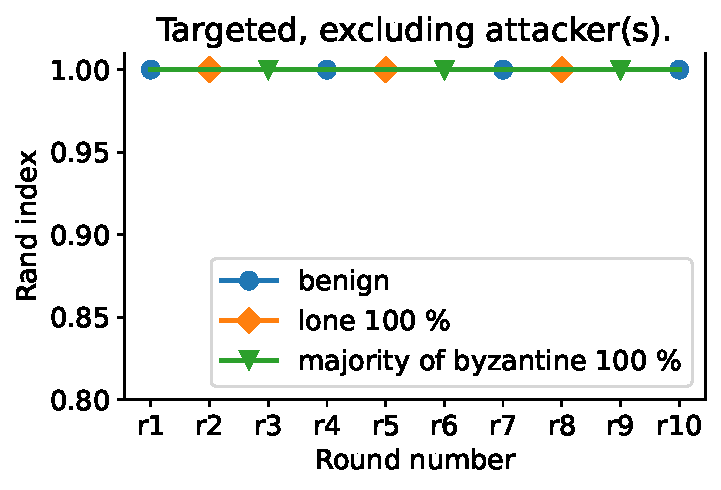
\includegraphics[width=0.47\linewidth]{figures/clustering/targeted_rand_no_attackers.pdf}
%     \quad
%     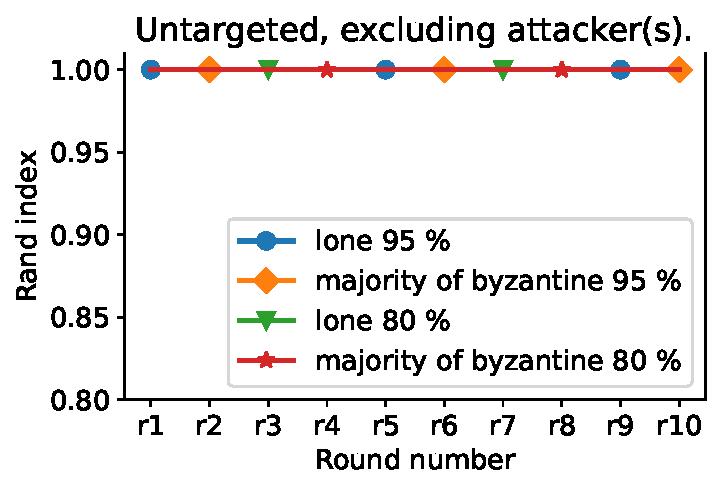
\includegraphics[width=0.47\linewidth]{figures/clustering/untargeted_rand_no_attacker.pdf}
%     \caption{
%       Clustering results compared with a partition with only benign participants.
%       The constant Rand Index of 1.0 means that all benign participants are correctly grouped according to their respective dataset, in all tested attacks.
%     }
%     \label{fig:rand_no_attackers}
%   \end{subfigure}

%   \begin{subfigure}[t]{\linewidth}
%     \centering 
%     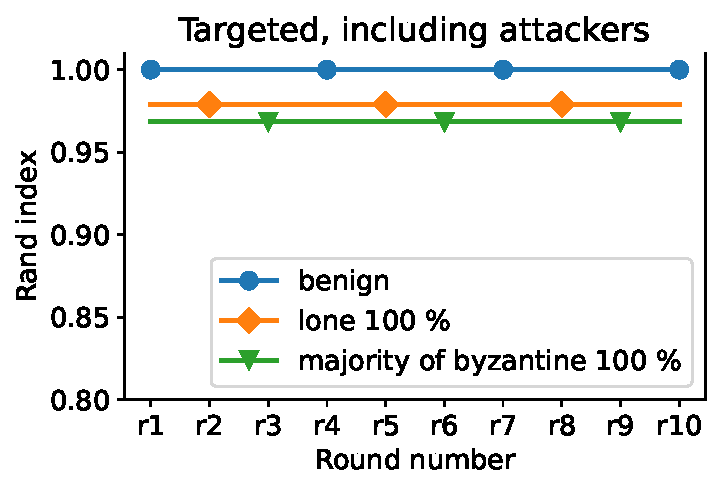
\includegraphics[width=0.47\linewidth]{figures/clustering/targeted_rand_attackers_separated.pdf}
%     \quad
%     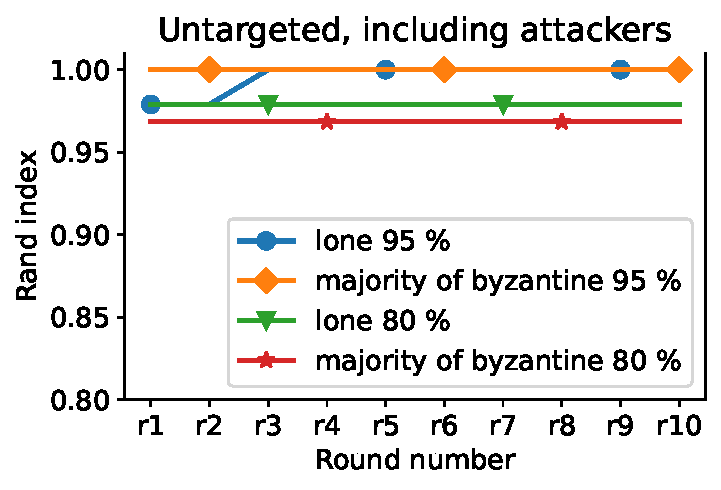
\includegraphics[width=0.47\linewidth]{figures/clustering/untargeted_rand_attackers_separated.pdf}
%     \caption{
%       Clustering results compared with a partition \textbf{with attackers grouped separately}.
%       A Rand Index of 1.0 (see untargeted attacks, \emph{noisiness} $\geq$ 95\%) means that attackers are separated from the legitimate participants, and thus cannot impact them.
%     }
%     \label{fig:rand_attackers_separated}
%   \end{subfigure}
  
%   \caption{
%     Evolution of the Rand Index over rounds, under various attack scenarios (see \Cref{sec:eval.methodo.scenarios}).
%     The Rand Index compares two partitions by quantifying how the different element pairs are grouped in each.
%     Two partitions are identical if all elements pairs are grouped or separated in the same way.
%     In this case, their Rand Index is 1.0.
%   }
%   \label{fig:rand_clustering}

% \end{figure}
% Scénarios avec des attaques. 
\subsubsection{Reputation system\label{sec:eval.results.reput}}
The reputation system weights participants inside each cluster, it aims at minimizing the weight of attackers without impacting too much the weight of benign participants. 
We first see in \Cref{fig:benign_targeted_non_expanded} that when there is no attack undergoing, all benign participants have an equal weight, underlining that the reputation system have almost no negative effect on benign participants. 
Furthermore, \Cref{fig:non_expanded_reputation}) illustrates that the reputation system is able to correctly penalize attackers, as long as they are a minority in their cluster. 
By construction, the reputation system detects the lone attacker from \Cref{fig:lone_loud_non_expanded} with a wider margin than colluding ones from \Cref{fig:byzantine_minority_loud_non_expanded}. 
Finally, the known limitation of the reputation system is apparent in \Cref{fig:byzantine_majority_loud_non_expanded}, attackers that become a majority inside a cluster gain precedence in weight and benign participants’ weight
drop. 

\begin{figure}[!t] 
  % Weights of the reputation system, before epansion.
  % Note: the images have unneeded blank space on the right.
  %       use trim+split to correct that.
  \centering
  \begin{subfigure}[t]{0.40\linewidth}
    \centering
    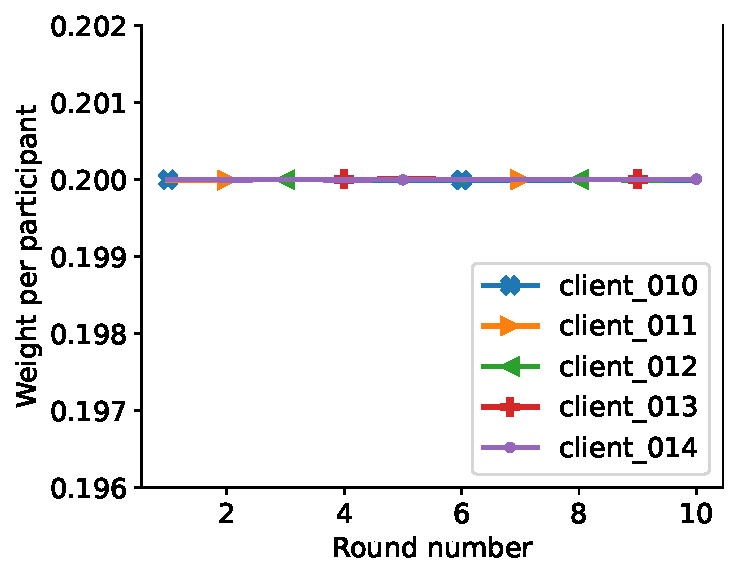
\includegraphics[trim=0 0 10pt 0,clip,width=\linewidth]{figures/reput/benign_non_expanded.pdf}
    \caption{Benign only, no difference.}
    \label{fig:benign_targeted_non_expanded}
  \end{subfigure}
  \quad 
  \begin{subfigure}[t]{0.40\linewidth}
    \centering
    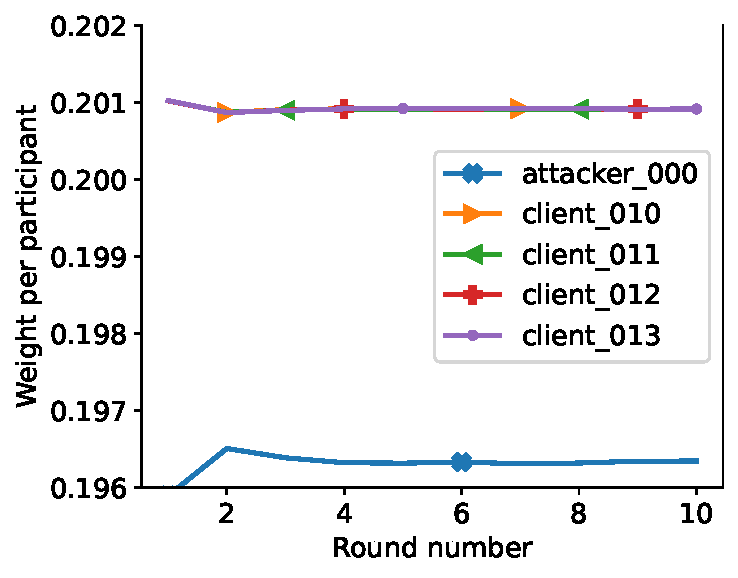
\includegraphics[trim=0 0 10pt 0,clip,width=\linewidth]{figures/reput/lone_loud_non_expanded.pdf}
    \caption{Lone attacker, clear identification.}
    \label{fig:lone_loud_non_expanded}
  \end{subfigure}

  \begin{subfigure}[t]{0.40\linewidth}
    \centering
    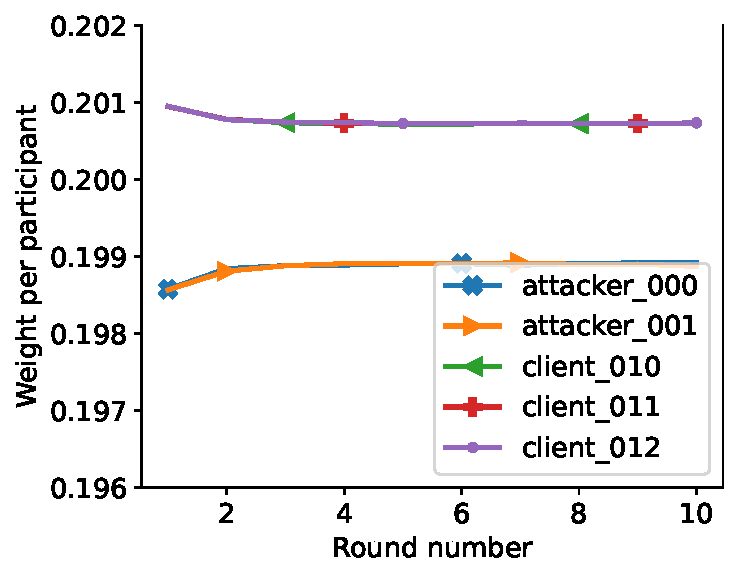
\includegraphics[trim=0 0 10pt 0,clip,width=\linewidth]{figures/reput/byzantine_minority_loud_non_expanded.pdf}
    \caption{Minority of Byzantines, less difference but still identifiable.}
    \label{fig:byzantine_minority_loud_non_expanded}
  \end{subfigure}
  \quad 
  \begin{subfigure}[t]{0.40\linewidth}
    \centering
    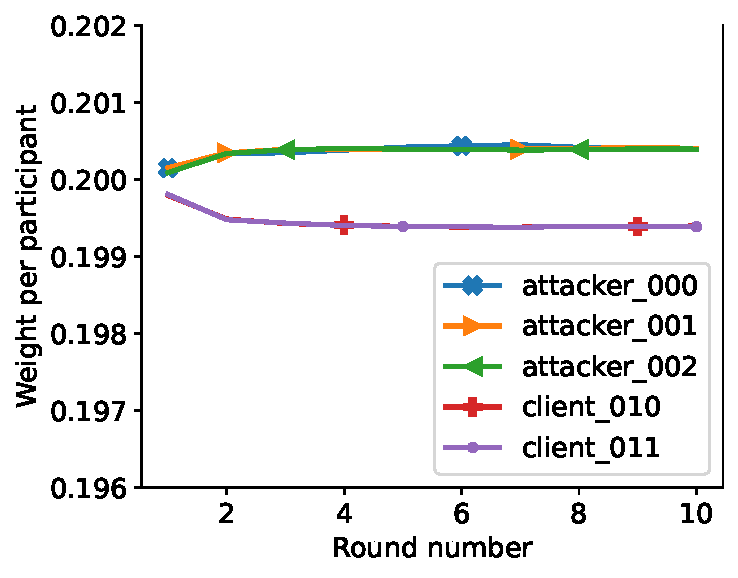
\includegraphics[trim=0 0 10pt 0,clip,width=\linewidth]{figures/reput/byzantine_majority_loud_non_expanded.pdf}
    \caption{Majority of Byzantines. Attackers gain precedence.}
    \label{fig:byzantine_majority_loud_non_expanded}
  \end{subfigure}
  \caption{
    Reputation weights $\weight$ (before expansion) given by the server for the participants of the poisoned cluster (targeted attack, 100\%) with varying number of attackers.  
    Attackers are correctly penalized when they are a minority, but gain precedence when they are the majority.}
  \label{fig:non_expanded_reputation}
\end{figure}
% Using a sigmoid function described in \Cref{sec:archi.reput}, we expand the weight differences between participants. 
One can notice the effect of the weight expansion by comparing the x-axis values between \Cref{fig:non_expanded_reputation} where weight expansion is voluntarily deactivated in the display to emphasize the difference between the different attackers' scenario, and \Cref{fig:redemption_decrease} where weight expansion is in display. 

Additionally, \Cref{fig:redemption_decrease} shows how the reputation system reacts to attackers that change their behavior over time. 
\Cref{fig:redemption_byzantine_min} feature a group of attackers going from 100\% \emph{noisiness}, to 0\%. 
They are forgiven after approximately four rounds after adapting their behavior, this rather short delay depends on the chosen $\lambda$ hyperparameter. 
On the contrary, a new attacker is detected and penalized after one round (\Cref{fig:increment_byzantine_min}), offering quick reaction to attacks. 


% \begin{figure}[!t] % REputation system weights expanded
%   \centering 

%   \begin{subfigure}[t]{.47\linewidth}
%     \centering 
%     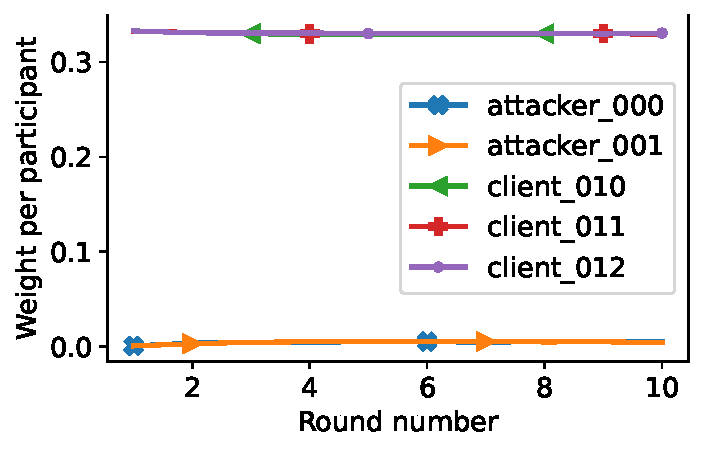
\includegraphics[trim=0 0 10pt 0,,clip,width=\linewidth]{figures/reput/byzantine_minority_loud_expanded.pdf}
%     \caption{
%       Minority of Byzantines (targeted attacks, $100\%$ \emph{noisiness}).
%       After weight expansion.
%     }
%     \label{fig:targeted_byzantine_minority_expanded_reputation}
%   \end{subfigure}
%   \quad
%   \begin{subfigure}[t]{.47\linewidth}
%     \centering 
%     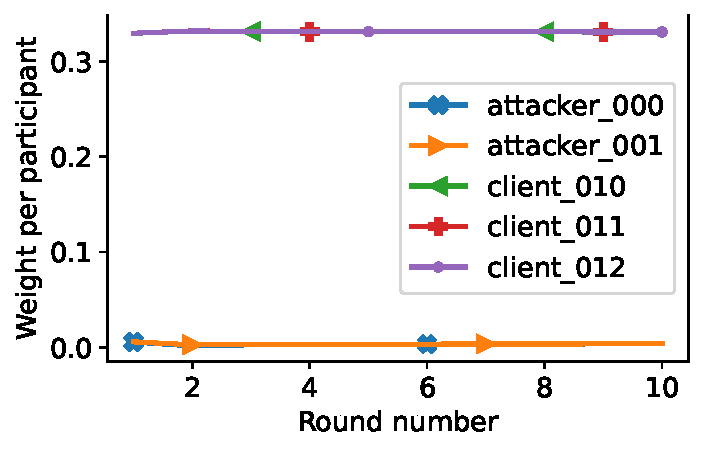
\includegraphics[trim=0 0 10pt 0,,clip,width=\linewidth]{figures/reput/untargeted_byzantine_minority_stealth_0_9.pdf}    
%     \caption{
%       Minority of Byzantines (untargeted attacks, $90\%$ \emph{noisiness}).
%       Before weight expansion.
%     }
%     \label{fig:untargeted_byzantine_minority_non_expanded_reputation}
%   \end{subfigure}

%   \caption{
%     Effect of the weight expansion function.
%     \Cref{fig:targeted_byzantine_minority_expanded_reputation} is the expanded counterpart of \Cref{fig:byzantine_minority_loud_non_expanded}, with the same scenario.
%     For \emph{loud} attacks (\Cref{fig:untargeted_byzantine_minority_non_expanded_reputation}), the difference between benign and attackers is already significant without expansion.
%   }
%   \label{fig:exploding_weights}
  
% \end{figure}

\begin{figure}[!t] % Reputation system redemption and late
  \centering 
  \begin{subfigure}[t]{.47\linewidth}
    \centering 
    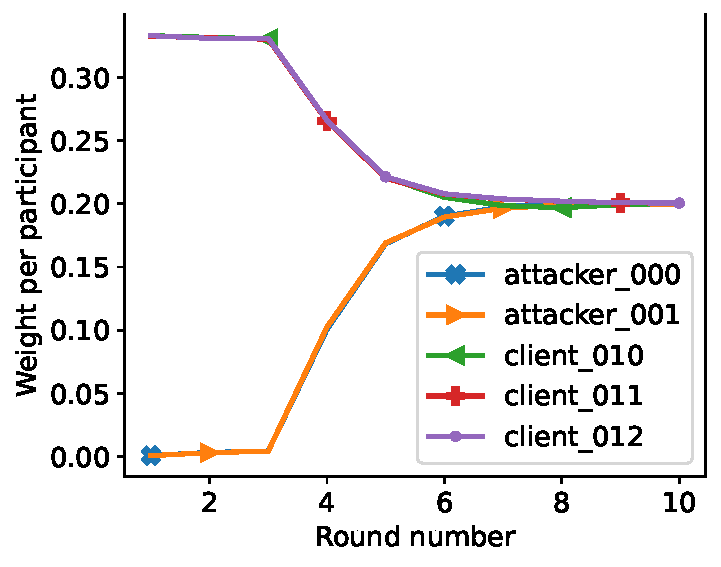
\includegraphics[trim=0 0 10pt 0,clip,width=\linewidth]{figures/reput/redemption_byzantine_min.pdf}    
    \caption{
      Attackers act with 100\% \emph{noisiness}, and become benign on round 3.
    }
    \label{fig:redemption_byzantine_min}
  \end{subfigure}
  \quad
  \begin{subfigure}[t]{.47\linewidth}
    \centering 
    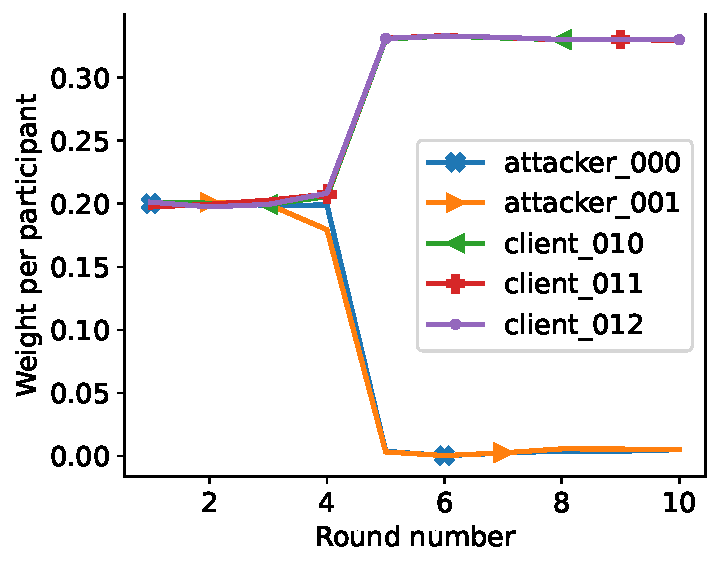
\includegraphics[trim=0 0 10pt 0,clip,width=\linewidth]{figures/reput/increment_byzantine_min.pdf}
    \caption{
      Attackers start benign, and increase \emph{noisiness} by 20\% each round when $r\geq3$.
    }
    \label{fig:increment_byzantine_min}
  \end{subfigure}
  \caption{
    Reputation weights $\weight$ (after expansion) per participant of the poisoned cluster (minority of Byzantines, targeted attack).
    Attackers are forgiven over time, and the reputation system reacts quickly to newly detected attackers.
  }
  \label{fig:redemption_decrease}

\end{figure}
%\subsubsection{Baseline comparison\label{sec:eval.results.baselines}}

\subsubsection{Comparative analysis \label{sec:eval.results.attacks}}


%\begin{table}[t]
%  % NOTE: résultats de FA_c extraits du notebook `exps/results/fedavg_per_dataset/processing.ipynb` (commit: TODO)
%      \centering
%          \caption{
%            Effects of different attack configurations (100\% \emph{noisiness}) on all baselines.
%            The attack success rate is computed over the targeted classes in targeted attacks, and over all samples otherwise (see \Cref{sec:eval.methodo.metrics}).
%            \texttt{TF} is \texttt{Trust-FIDS}, \texttt{FG} is \texttt{FoolsGold}, and \texttt{FA} is \texttt{FedAvg} (on \emph{all} participants).
%          \label{tbl:baselines_results}}
%      \bigskip
%      \setlength\tabcolsep{1ex}
%      \begin{tabular}{ll|rrr|crrrc}
%          \toprule % ---------------------------------
%          \multicolumn{2}{c|}{\multirow{2}{*}{\textbf{Attack type}}} & \multicolumn{3}{c|}{\textbf{Mean accuracy} (\%)} & \multicolumn{5}{c}{\textbf{Attack success rate} (\%)} \\
%          & & \multicolumn{1}{c}{\texttt{TF}} & \multicolumn{1}{c}{\texttt{FG}} & \multicolumn{1}{c}{\texttt{FA}}  & &\multicolumn{1}{c}{\texttt{TF}} & \multicolumn{1}{c}{\texttt{FG}} & \multicolumn{1}{c}{\texttt{FA}} & \\
%          \midrule
%          & Benign & \textbf{99.07} & 55.04 & 79.49  & & -  & - & - & \\
%          \midrule % ---------------------------------
%          % TARGETED ATTACKS
%          \multicolumn{2}{l|}{\textbf{Targeted}} & & & & & & & & \\
%            & Lone & \textbf{99.06} & 60.51 & 77.38 & & \textbf{0.00} & 93.82 & 6.73 &  \\
%            & Minority of Byzantines & \textbf{98.96} & 54.64 & 78.48 & & \textbf{0.00} & 2.97 & 9.99  &\\
%            & Majority of Byzantines & \textbf{98.28} & 85.10 & 79.40 & & 79.39 & \textbf{8.01} & 17.65 & \\
%          \midrule % ---------------------------------
%          % UNTARGETED ATTACKS
%          \multicolumn{2}{l|}{\textbf{Untargeted}} & & & & & & & &\\
%            & Lone & \textbf{98.96} & 49.56 & 78.38 & & \textbf{0.08} & 99.89 & 54.70 &\\
%            & Minority of Byzantines & \textbf{98.98} & 49.67 & 72.47 & & 0.10 & \textbf{0.04} & 44.53 &\\
%            & Majority of Byzantines & \textbf{98.96} & 69.09 & 81.87 & & \textbf{0.08} & 38.98 & 59.49 &\\          
%          \bottomrule % ---------------------------------
%      \end{tabular}
%  
%  %\end{minipage}      
%  \end{table}

\begin{table}[t]
  % NOTE: résultats de FA_c extraits du notebook `exps/results/fedavg_per_dataset/processing.ipynb` (commit: TODO)
      \centering
          \caption{
            Effects of different attack configurations (100\% \emph{noisiness}) on all baselines.
            The attack success rate is computed over the targeted classes in targeted attacks, and over all samples otherwise (see \Cref{sec:eval.methodo.metrics}).
            \texttt{TF} is \texttt{Trust-FIDS}, \texttt{FG} is \texttt{FoolsGold}, $\texttt{FA}_a$ is \texttt{FedAvg} (on \emph{all} participants), and $\texttt{FA}_c$ is \texttt{FedAvg} ideally clustered per dataset.
            The ``attack success rate'' of benign runs is provided as a baseline.
            \thecontrib's limiting scenario is marked $\ddagger$.
          \label{tbl:baselines_results}}
      \bigskip
      \setlength\tabcolsep{1ex}
      \begin{tabular}{ll|rrrr|rrrr}
          \toprule % ---------------------------------
          \multicolumn{2}{c|}{\multirow{2}{*}{\textbf{Attack type}}} & \multicolumn{4}{c|}{\textbf{Mean accuracy} (\%)} & \multicolumn{4}{c}{\textbf{Attack success rate} (\%)} \\
          & & \multicolumn{1}{c}{\texttt{TF}} & \multicolumn{1}{c}{\texttt{FG}} & \multicolumn{1}{c}{$\texttt{FA}_a$} & \multicolumn{1}{c|}{$\texttt{FA}_c$} & \multicolumn{1}{c}{\texttt{TF}} & \multicolumn{1}{c}{\texttt{FG}} & \multicolumn{1}{c}{$\texttt{FA}_a$} & \multicolumn{1}{c}{$\texttt{FA}_c$} \\
          \midrule % ---------------------------------
          % TARGETED ATTACKS
          \multicolumn{2}{l|}{\textbf{Targeted}} & & & & & & & & \\
            & Benign & \textbf{99.07} & 55.04 & 79.49 & 99.24 & \textbf{0.0}  & 5.17 & 5.10 & 0.09 \\
            & Lone & \textbf{99.06} & 60.51 & 77.38 & 99.22 & \textbf{0.00} & 93.82 & 6.73 & 0.45 \\
           & Minority of Byzantines & \textbf{98.96} & 54.64 & 78.48 & 98.33 & \textbf{0.00} & 2.97 & 9.99 & 53.40 \\
            $\ddagger$ & Majority of Byzantines & \textbf{98.28} & 85.10 & 79.40 & 98.22 & 73.39 & \textbf{8.10} & 17.65 & 59.36 \\
          \midrule % ---------------------------------
          % UNTARGETED ATTACKS
          \multicolumn{2}{l|}{\textbf{Untargeted}} & & & & & & & & \\
            & Benign & \textbf{99.07} & 55.04 & 79.49 & 99.24 & 0.09  & 0.39 & 33.30 & \textbf{0.06} \\
            & Lone & 98.96 & 49.56 & 78.38 & \textbf{99.22} &\textbf{0.08} & 99.89 & 54.70 & 0.12 \\
            & Minority of Byzantines & \textbf{98.98} & 49.67 & 72.47 & 97.69 & 0.10 & \textbf{0.04} & 44.53 & 6.26 \\
            & Majority of Byzantines & \textbf{98.96} & 69.09 & 81.87 & 75.66 & \textbf{0.08} & 38.98 & 59.49 & 94.36 \\          
          \bottomrule % ---------------------------------
      \end{tabular}
  
  %\end{minipage}      
  \end{table}

We compare \thecontrib with selected baselines under various attack scenarios in \Cref{tbl:baselines_results}. 
First, the results highlight the relevance of clustering in  \emph{practical \gls{niid}} use cases, as attacks are confined to the cluster attackers have been assigned to.
This is particularly visible in the accuracies of \thecontrib and $\texttt{FedAvg}_c$, which both maintain high accuracy overall, even for targeted attacks in majority where \thecontrib starts to falter. 
However, since \texttt{FedAvg} does not implement any mitigation strategy, its performance quickly degrades, especially by colluding attackers.

%We compare \thecontrib with selected baselines under various attack scenarios in \Cref{tbl:baselines_results}. 
%First, the results highlight the relevance of clustering in  \emph{practical \gls{niid}} use cases, as attacks are confined to the cluster attackers have been assigned to.
%This is particularly visible in the high accuracy of \thecontrib under the different attack scenarios.
%Even with a \emph{majority of Byzantines} performing targeted attacks, where \thecontrib starts to falter, the accuracy remains high since the other clusters are unaffected.
%
%Additionally, we test the attack success rate of \texttt{FedAvg} under the \emph{majority of Byzantines} scenario when all participants are trained on Bot-IoT.
%Attacks are effective at 59.37\% when targeted, and 94.37\% when untargeted, whereas \thecontrib obtains 73.39\% and 0.8\%, respectively.
%Since \texttt{FedAvg} does not implement any mitigation strategy, it is highly impacted, while not favoring attackers, in contrast to \thecontrib in the specific case of a majority of colluding targeted attackers.
%\texttt{FedAvg} with all participants, on the other hand, obtains consistently poor results, because of the absence of clustering.

The results in \Cref{tbl:baselines_results} also emphasize on \texttt{FoolsGold}'s unsuitability for \emph{practical \gls{niid}} use cases, where groups of participants sharing similar distributions can exist.
Especially in a \emph{lone attacker} scenario, any groups of similar participants are considered as colluding attackers and penalized, leading to high attack success rate, as only the attacker is considered as legitimate.
Similarly, in a \emph{minority of Byzantines} scenario, \texttt{FoolsGold} penalizes all the other clusters, leading to a model trained on Bot-IoT only.

Overall, \thecontrib shows the most consistent results, with high accuracy and low attack success rate in most scenarios, only failing against a majority of colluding participants.  
This limitation is also illustrated in \Cref{fig:trustfids_accuracy_missrate_distribution}, with a steeper drop in accuracy and miss rate when attackers outnumber benign participants in one cluster.
However, the metric distribution over the participants shows that the other clusters remain unaffected, and that the majority of benign participants continues to perform well.
This limitation is further mitigated when attackers are \emph{noisy} enough, as mentioned in the clustering analysis, since they are placed in their own cluster.
The results of \Cref{tbl:baselines_results} illustrates this, with an especially low attack success rate in \emph{untargeted} attacks, even in the \emph{majority of Byzantines} scenario. 


%In the targeted minority of Byzantine scenario, only participants from the Bot-IoT dataset are kept, while those coming from other datasets are all discarded.
%This leads to a model that is specialized on this dataset, and thus shows great results on the targeted class but an accuracy worse than \texttt{FedAvg} overall.

%Finally, in the targeted Byzantine scenario with a \emph{majority} of attackers, malicious participants are dropped and all benign are kept, leading to slightly better results than a benign \texttt{FedAvg}.
% pathological non-IID inadequate for intrusion detection (benign + attack necessary), fools gold doesn't perform well in this setting either.

%We used the following hyperparameters for the clustering: distance were measured using cosine~similarity, see \Cref{eq:cosin_sim} and the hierarchical clustering threshold is equal to 1/4th of the mean initial inter-distance. 




%\subsubsection{Resistance to attacks\label{sec:eval.results.attacks}}
% \Cref{tbl:baselines_results} presents the effect of the poisoning with varying number of attackers on the different baselines. 

% Pm : suppression des lignes dessous car exposées dans metrics et dans la légende.
% Since we mostly want to know if benign participants can be poisoned by attackers, we strip attackers from the results and only keep benign participants.  
% We then show the average accuracy of all benign participants.
% The Miss column is the average miss rate of participants as exposed in \Cref{sec:eval.methodo.metrics}.
% A complete statistic overview of these results for \thecontrib is  visually exposed in \Cref{fig:trustfids_accuracy_missrate_distribution}.
% We can see in \Cref{tbl:baselines_results} that \thecontrib successfully stops targeted attacks as long as the attackers are a minority inside their cluster: the miss rate for the lone and minority of Byzantine does not increase compared to the benign case. % deja dit, pas autant de détails
% The tipping point is when attackers outnumber legitimate participants: here, a majority of the targeted labels are misclassified. %déjà dit
% This switch can also be seen in \Cref{fig:trustfids_accuracy_missrate_distribution} with a steep degradation of the accuracy and the missrate for the participants in the targeted cluster once attackers become the majority in this cluster. 
% Also illustrated in \Cref{fig:trustfids_accuracy_missrate_distribution} however is the fact that the clients placed in the others clusters are unaffected by this event, underlining the clustering ability to limit the impact of a successful attack. 
% For untargeted attacks, we don't observe a switch when attackers become the majority. % table
% As further explained in \Cref{sec:eval.results.cluster}, untargeted attackers are noisy enough to be placed in a cluster of their own and thus have no effect on other participants. % déjà dit
% We can also see that for both untargeted and targeted attacks, the mean accuracy decreases with the number of attackers. % où ?
% Since we work with a fixed amount of data for each dataset, introducing attackers reduces the amount of data available for benign participants, which decreases their performance. % pas le cas dans nos exps...




\begin{figure}[!t]
  %\centering 
  \begin{subfigure}[t]{1.0\linewidth}
    \centering 
    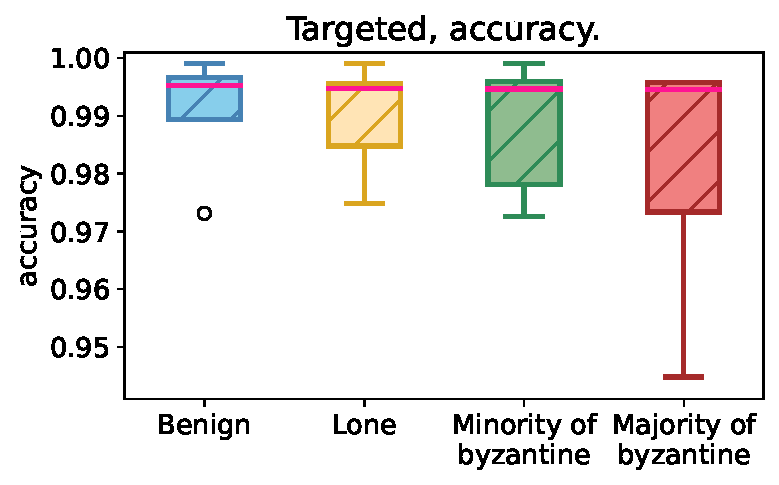
\includegraphics[width=0.47\linewidth]{figures/poisoning/trusfids_targeted_acc_all_distibutions.pdf}    
    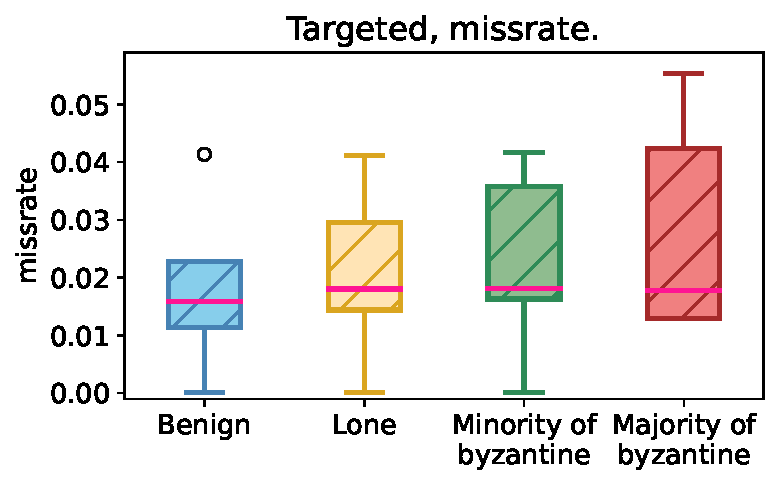
\includegraphics[width=0.47\linewidth]{figures/poisoning/trusfids_targeted_missrate_all_distibutions.pdf}   
\end{subfigure}
  \caption{
    % \thecontrib's client distribution of miss rates in different attack scenarios. 
    % The accuracy and missrate suddenly drop when attackers become the majority. 
    % Note that this effect only applies to some clients as the clients placed in others clusters are unaffected by the poisoning.
    \thecontrib's metric distribution among participants in different attack scenarios (targeted attacks, 100\% \emph{noisiness}).
    The accuracy's and miss rate's lower bounds suddenly drop when attackers outnumber benign participants in the affected cluster.
    Indeed, clients in other clusters are unaffected by the poisoning.
  }
  \label{fig:trustfids_accuracy_missrate_distribution}
  
\end{figure}
\section{Discussion}\label{sec:discussion}

\thecontrib shows versatility in how it addresses the complex problem of identifying attackers in heterogeneous contexts.
However, the interpretation of the presented results is limited to our small-scale \gls{nids} use case.
In this section, we discuss the limitations and potential consequences of our architecture and propose research directions to close these gaps. 

\paragraph{Generalizability.} 

While the experiments are only conducted on intrusion detection datasets, \thecontrib's design could be used in different use cases regarding the following conditions: (1) parametric local models whose parameters can be aggregated using \gls{fl}, and (2) local testing sets and relevant metrics allowing participants to evaluate the others’ models.
Since the \gls{nids} use case induces a focus on malicious samples (\ie \emph{positive} values), we choose the F1-score as input for both the clustering and reputation, as it emphasizes on false positives and false negatives.
Other use cases might find using the loss of a model more relevant, especially for similarity measurements.
Further, \thecontrib's resilience against practical \gls{niid} settings makes it also relevant for safety objectives, where negligent participants can also exist.

\paragraph{Scalability and performance.}

The focus on small-scale collaboration (\ie a few dozens of participants) makes the overhead of the \emph{cross-evaluation} step (\Cref{sec:archi.xeval}) practical, and justifies the absence of performance-related metrics in this paper.
However, it makes \thecontrib in its current state unsuitable for highly distributed scenarios.
Each round, clients evaluate $|P|$ additional models, which scales linearly with the number of clients.
Two new communications are also introduced, one to send the models and one to collect the evaluations.
The size of the former also grows linearly with $|P|$, as the models of all participants must be distributed.
Likewise, we exclude execution-related performance evaluation such as training time, CPU overhead, or bandwidth consumption.
%We leave the feasibility of \thecontrib to future works, and emphasize on its ability to maintain high accuracy.
%This makes \thecontrib more suited for small-scale collaboration, such as our \gls{cids} use case.
It opens the way to interesting research directions on how to implement and scale \thecontrib while guarantying its properties.


% // Removed because it only restates the findings of the Results section
% \paragraph{Attack mitigation.} 

% Throughout this paper, we emphasize on \thecontrib's versatility, as it can cope with multiple attack scenarios simultaneously.
% However, a group of numerous attackers with evaluations close enough to benign participants might be grouped with them.
% If they represent the majority of the newly created cluster, they will be favored by the reputation system.
% Therefore, combining \thecontrib with additional mitigation strategies inside clusters, more geared toward the detection of numerous malicious participants, is a relevant research direction.
\paragraph{Evaluation poisoning.}
%While not covered in the experiments, 
Attackers could try to poison the evaluations that they provide on other participants to abuse the system.
%One possibility for attackers would be to change arbitrarily the evaluations that they provide on other members to abuse the system. 
However, the implementation presented in \Cref{sec:eval.methodo} implies that attackers poison both their training and testing sets.
Consequently, the evaluations they produce on other participants are directly affected.
We thus expect the system to cope with arbitrary poisoning similarly to data poisoning: either by placing the attackers in a different cluster because of their dissimilarity, or by penalizing their reputation. 

% \paragraph{Information disclosure.}
% Because \thecontrib shares models with the other participants to obtain feedbacks, it can be argued that it revels more information about the participants.
% This is limited to the participants' models, which are shared without identifiers.
% However, since clients also receive the global model of their cluster, they can try to estimate the models that belong to their cluster.
% This remains challenging, as the models are weighted using the reputation score of the participants, which are only available to the server.
% Comparing the privacy impact of \thecontrib with those of simpler approaches like \texttt{FedAvg} represents interesting research directions.

\section{Conclusion}\label{sec:conclu}
% 1 sentence : name of what we did + a general overview. 
In this paper, we introduced \thecontrib, a federated learning architecture that effectively mitigates poisoning attacks, even with heterogeneous data-distributions.
% 1-2 sentences : Assumptions made for the work. Could we validate them ?
Our approach is built on the assumption that heterogeneous participants can be grouped based on the similarity between their data distribution.
% Assumption : In 
 % that share similarities, we have chosen to group participants together.
% Methodo 
To test this assumption, we instantiated four groups of clients based on four different public datasets in a way that each client has data coming from a single dataset. 
% 3-4 sentences main results
We introduced a cross-evaluation scheme that allows participants to estimate their pairwise similarities. 

Using the similarity between the participants' evaluations, we manage to rebuild the initial participant distribution using hierarchical clustering. 
We further designed a reputation system based on the cross-evaluation results.
Our reputation system uses the perceived similarity of participants and their cumulated past results to give a score to each participant inside a cluster.     
We show that this reputation system can distinguish attackers from benign participants as long as attackers remain the minority in a cluster. 
% By accentuating the reputation differences, we obtain aggregation weights that are used to build a different model for each cluster. 
Our process greatly reduces the impact of attackers. 
We compared our work to \texttt{FoolsGold} and \texttt{FedAvg}, which highlighted the versatility of \thecontrib.
% As future works, noting that \thecontrib and \texttt{FoolsGold} produce complementary results, we would like to investigate whether an approach that opportunistically switch between the two is possible. 
%
% mop : I would rather write something like "The next step for continuing our work is..."
%
% mop : However, the risk is always: why didn't you do it yet? Why should we accept such preliminary work? Therefore it is good to emphasize that the result is already great. However, this would be a follow-up point for other researchers.
% mop: edited it accordingly.
%
%As possible next steps into the direction of the presented research, introducing more heterogeneity inside the different group of participants by dropping one or multiple classes of attacks could be an interesting next step. 

Finally, overcoming \thecontrib's limited scalability paves the way towards interesting research directions, as trust is also a requirement in cross-device settings.
Moreover, being able to remove the central server dependency is a key step towards a truly decentralized, trustworthy, and privacy-preserving \gls{cids}.
% \section*{Acknowledgements\label{sec:ack}}

% Funding...

% Author contrubutions: ....

% Apart from the first authors, the order of appearance has been chosen alphabetically.

\printbibliography

\section*{Appendix\label{sec:annexes}}

%\vspace{-1cm}
%\begin{table}[H]
%    \centering
%    \caption{\label{tbl:notations}Notations}
%    % As a general rule:
%    % 1) sets and sequences shall be defined in uppercase
%    % 2) samples or individual entities shall be expressed in lowercase
%    \begin{tabularx}{\columnwidth}{l|X}
%        \toprule % ---------------------------------
%        \textbf{Notation}  & \textbf{Description} \\
%        \midrule % ---------------------------------
%        $\p$                                                                & Participant $i$ \\
%        $\d$                                                                & Local dataset of participant $p_i$ \\
%        $D = \bigcup_{i=1}^n d_i$                                           & Union of all local datasets \\
%        $n$                                                                 & Number of participants \\
%        $P = \{\p\}_{i \in \llbracket 1,n \rrbracket}$                      & Set of all participants \\
%                  
%        $\c$                                                                & Cluster $k$ at round $r$\\
%        $\center$                                                           & Cluster $k$ center at round $r$\\
%        $m^r$                                                               & Number of clusters at round $r$ \\
%        $\C = \{ C^r_i\}_{i \in \llbracket 1 ,m^r \rrbracket}$              & Set of clusters at round $r$ \\
%        $\dist$                                                             & Distance from cluster $k$ and $\ell$ centers at round $r$ \\
%        $\w$                                                                & Local model of participant $i$ at round $r$\\
%        $\W = (w_i^r)_{i \in \llbracket 1,n \rrbracket}$                    & All local models from participants at round $r$\\
%        $\wbar$                                                             & Global model for cluster $c_k^r$ at round~$r$\\
%        $\Wbar = (\wbar)_{k \in \llbracket 1,|\C| \rrbracket }$             & All global models at round $r$ \\                               
%        $e_{i,j}^r $                                                        & Evaluation of $w_j^r$ using $p_i$ local dataset $d_i$ \\
%        $\E = [e_{i,j}^r]_{i,j \in \llbracket 1,n \rrbracket}$              & Matrix of all evaluations at round $r$; of size $n \times n$ \\
%        $\issue = (e_{i,j}^r)_{j \in \llbracket 1,n \rrbracket}$            & $p_i$ evaluation on every participant at round $r$ \\
%        $\rece = (e_{i,j}^r)_{i \in \llbracket 1,n \rrbracket}$             & Participants evaluations on $\p[j]$ at round $r$ \\
%        \bottomrule % ---------------------------------
%    \end{tabularx}
%\end{table}

\begin{algorithm}[t]
\caption{
    \thecontrib.
    $R$ is the number of rounds, $\beta$ the local batch size, $\eta$ the learning rate, $\mathcal{E}$ the number of epochs, and $\lambda$ a loss function.\label{alg:xeval}}
\begin{small}
\begin{algorithmic}[1]
    \Require $P$

    \With{$r \gets 0$}
        \State \( \C \gets \{ P \}                  \)
        \State \( \Wbar \gets (\Call{Random}{\ })   \)
    \EndWith
    \Statex
    \For{$r \gets 1,\dots,R $}
        \LComment{Step (1): model training}
        \ForAll{$p_i \in P$ \textbf{in parallel}}
            \State $k \gets \Call{GetCluster}{p_i, \C}$
            \State $\w \gets \Call{ClientFit}{p_i, \wbar}$
        \EndFor
        \Statex
        \State \( \W \gets (\w)_{i \in n \llbracket 1,n \rrbracket} \) 
        \Statex
        \LComment{Step (2): cross-evaluation}
        \ForAll{$p_i \in P$ \textbf{in parallel}} 
            \State $(\e) \gets \Call{ClientEvaluate}{p_i, \W}$
        \EndFor
        \State \( \E_{[i,j]} = [e_{i,j}^r]_{i,j \in \llbracket 1,n \rrbracket} \)
        \Statex
        \LComment{Step (3): parameters aggregation}
        \State \( \C \gets \Call{ComputeClusters}{\E} \)     \Comment{See:~\Cref{sec:archi.cluster}}
        \ForAll{$  \c \in \C $}
            \State \( (\rho_i^r) \gets \Call{ComputeReput}{\E, \C} \)   \Comment{See:~\Cref{sec:archi.reput}}
            \State \( \Wbar \gets \frac{1}{|\c|} \sum_{i=0}^|\c| \w \)
        \EndFor
    \EndFor

    \Statex % Client-side model training
    \Function{ClientFit}{$p$, $\omega$} \Comment{On client.}
        \For{$ i \gets 1,\dots,\mathcal{E} $}
            \ForAll{$ b \in \Call{split}{\d, \beta} $}
                \State \( \omega \gets \omega \nabla \lambda(\omega;b) \) \Comment{See:~\Cref{sec:problem.cids}}
            \EndFor
        \EndFor
        \\
        \State \Return $\omega$
    \EndFunction

    \Statex % Client-side evaluation
    \Function{ClientEvaluate}{$p$, $\Omega$} \Comment{On client.}
        \ForAll{$ \omega_j \in \Omega $}
            \State \( \e \gets \Call{Eval}{\omega, \d} \)
        \EndFor
        \State \Return $(\e)_{i,j \in [\![ 1,n ]\!]}$
    \EndFunction
\end{algorithmic}
\end{small}
\end{algorithm}

% \subsection{Reputation system\label{sec:annexes.reput}}
% This section provides a more in-depth look at the reputation system exposed in~\ref{sec:archi.reput}.  
% The reputation of a participant $\p$ is based on its received evaluations, $\rece[i]$ which are continuous over $[0,1]$.
% For this reason, and similar to~\citet{fung_dirichlet-based_2011}, we choose to use a reputation system based on the multivalued Dirichlet probability distribution for trust modeling. 
% Using a multivalued distribution allows us to discretize $\rece[i]$ into a set of $q$ possible values $\mathcal{E} = \{\varepsilon_1, \varepsilon_2, \ldots, \varepsilon_q\}$.  
 
%  % Aggregation step relies on weights that are scalar values representing the importance given to a participant's parameters in the aggregation. Contributions are weighted based on the participants' reputation score, built using the evaluation matrix $\E$ as an input, and focusing on the received evaluations.
% %These are received by a specific participant for its model parameters, and made by other participants using their own datasets. 
% % Evaluations of participant \(p\) are computed by other participants on their local datasets by applying \(p\)'s model parameters.

% % The evaluation metric of a participant is continuous over $[0,1]$ but Dirichlet distributions are multivalued.
% % Consequently, we first
% A Dirichlet distribution on the outcome of an unknown event is usually based on the combination of an initial belief vector and a series of cumulative observations~\cite{fung_dirichlet-based_2011}. 
% Since the results from a complete first round of cross evaluation are already available when reputation is first assessed, we do not need to use an initial belief vector to bootstrap. 
% Following the notation used by~\citet{fung_dirichlet-based_2011}, we denote  by $\vec{\gamma} = \{\gamma_{1},\gamma_{2},\ldots,\gamma_{q}\}$ the cumulative previous evaluations: $\gamma_{2}=3$ means that three evaluations in $\rece$ had values bounded by $[\frac{2,5}{q},\frac{3,5}{q}[$.

% We then note $\Prob = {\prob[\varepsilon_1],\prob[\varepsilon_2], \ldots, \prob[\varepsilon_q]}$ the probability distribution vector for the received evaluation of a participant, where $\sum_{s=1}^{q}\prob[\varepsilon_s] = 1$.
% Leveraging the previous evaluations $\vec{\gamma}$, the probability $\cond[\varepsilon_s]$ is given by Eq.~\ref{eq:s_knowing_gamme}, 
% %\begin{equation}\label{eq:s_knowing_gamme}
% %    \cond = \frac{\gamma_{s}}{\gamma_{0}},
% %\end{equation}
% where $\gamma_0$ is the number of evaluations previously received by $\p$, as shown in~\Cref{eq:gamma_sum}.
% %\begin{equation}\label{eq:gamma_sum}
% %    \gamma_0 = \sum_{s=1}^{q}{\gamma_{s}}.
% %\end{equation}

% \vspace{-1cm}
% \begin{multicols}{2}
% \begin{equation}\label{eq:s_knowing_gamme}
%     \cond = \frac{\gamma_{s}}{\gamma_{0}},
% \end{equation}\break
% \begin{equation}\label{eq:gamma_sum}
%     \gamma_0 = \sum_{s=1}^{q}{\gamma_{s}}.
% \end{equation}
% \end{multicols}

% We want to limit the ability of potential malicious participants to divert the use of the reputation system by badmouthing another participant, or by artificially raising their own ratings.
% We thus weight the issued evaluation $\issue[j]$ of a participant $\p[j] \in \c$ according to its similarity with other cluster members\cite{xiong_peertrust_2004}. 
% The similarity is measured using the standard deviation between $\p[j]$ and its cluster center $\center$, as shown in~\Cref{eq:standard_deviation}.

% % Pour ce second cas d'usage ne vaudrait-il pas mieux prendre la similarité des votes émis sur le participant qu'on est en train de pondérer plutôt que sur l'ensemble des participants ? 
% % C'est une adaptation de peertrust qui pondère les votes en comparant les votes émis des deux participants. L'expliquer ? Justifier la diff ?

% \begin{equation}\label{eq:standard_deviation}
%     \sigma_j^r = sim(\issue[j],\center) = 1 - \sqrt{
%         \frac{
%             \sum_{i=1}^{|\P|}{
%                 {(\e[j][i] - \mu^r_{k,i})}^{2}
%             }
%         }
%         {
%             |\P|
%         }
%     }.
% \end{equation}


%We then leverage a forgetting factor $\lambda \in [0,1]$ to reduce the importance of evaluations from older rounds. 
%This necessary because we need to take past contributions into account to limit attacks phased over multiple rounds, while preventing past mistakes from permanently impacting a participant. 
%The reputation $\rep$ of a participant $\p$ at round $r$ based on the prior knowledge $\gamma^r_i$ of this participant is given by \Cref{eq:reputation_history}.

%In order to prevent attacks phased over multiple rounds, while preventing past mistakes from permanently impacting a participant, we leverage a forgetting factor $\lambda \in [0,1]$. The reputation $\rep$ of a participant $\p$ at round $r$ based on the prior knowledge $\gamma^r_i$ of this participant is given by \Cref{eq:reputation_history}.
%%
%%\begin{equation}\label{eq:reputation_history}
%%    \rep = \sum_{\kappa=1}^{r}\lambda^{r-\kappa}\sigma_i^\kappa\gamma_i^{\kappa}.
%%\end{equation}
%%
%Note that a small $\lambda$ gives more importance to recent evaluations: $\lambda=0$ only considers the last round while $\lambda=1$, considers all round with equal weight.  
%%This parameter stays constant for all rounds, we chose to fix it at 0.9 following the value used by \citet{fung_dirichlet-based_2011}.
%Based on $\rep$, let $\weight$ be the weight of $\w$ for aggregation in $\wbar$ is given by \Cref{eq:weight_computation}, where $\weight$ is the weight of $\w$, the model from $\p$, that will be used during the aggregation of $\wbar$ (see \Cref{alg:xeval}~Step~(3) in~\Cref{sec:annexes}).
%
%% \begin{equation}\label{eq:weight_computation}
%%    \weight = \frac{\rep}{\sum_{j=1}^{\c}\rep[j]},
%% \end{equation}
%
%\vspace{-1cm}
%\begin{multicols}{2}
%\begin{equation}\label{eq:reputation_history}
%    \rep = \sum_{\kappa=1}^{r}\lambda^{r-\kappa}\sigma_i^\kappa\gamma_i^{\kappa}.
%\end{equation}\break
%\begin{equation}\label{eq:weight_computation}
%    \weight = \frac{\rep}{\sum_{j=1}^{\c}\rep[j]},
%\end{equation}
%\end{multicols}
%  
%We then widen the gap between each cluster weights using their deviation to the average and passing them to a sigmoid function. 
%We use the normal distribution cumulative density function as the sigmoid function, adjusting the $\sigma$ parameter in order to penalize attackers without having too much impact on benign participants. 
% Schéma du placement des poids sur la courbe ? Réf vers cette figure ? 

%%%%%%%%%%%%%%%%%%%%%%%%%%%%%%%%%%%%%%%%%%%%%%%%%%%%%%%%%%%%%%%%%%%%%%%%%%%%%%%%
%               DOCUMENT END
%%%%%%%%%%%%%%%%%%%%%%%%%%%%%%%%%%%%%%%%%%%%%%%%%%%%%%%%%%%%%%%%%%%%%%%%%%%%%%%%

% \defaultprintbib % print the bibliography



\end{document}
%%
%% End of file `main.tex'.